\documentclass[output=paper,hidelinks]{langscibook}
\ChapterDOI{10.5281/zenodo.10185964}
\title{Glue semantics}
\author{Ash Asudeh\affiliation{University of Rochester}}
\abstract{\glues\ is a general framework for semantic composition and the syntax--semantics interface. It  assumes an autonomous syntax and therefore needs to be paired with some syntactic theory. Here the focus is on LFG as the syntactic theory. The \glue\ logic, a fragment of linear logic, is presented first. This highlights the resource sensitivity of semantic composition in \glue. Second, \glue\ is presented without reference to LFG or any other syntactic theory. This highlights \glue's property of flexible composition. Third, the syntax--semantics interface is considered. This highlights \glue's autonomy of syntax and serves as a way to compare and constrast \glue\ with well-known alternatives. Fourth, \glue\ is paired with LFG (\lfgglue), which highlights another important property of the theory, syntax/semantics non-isomorphism. Lastly, a number of particular phenomena are briefly reviewed and their analyses sketched: quantifier scope, modification, tense, events, argument structure, multiword expressions, and anaphora.}

\IfFileExists{../localcommands.tex}{
   \addbibresource{../localbibliography.bib}
   \addbibresource{thisvolume.bib}
   % add all extra packages you need to load to this file

\usepackage{tabularx}
\usepackage{multicol}
\usepackage{url}
\urlstyle{same}
%\usepackage{amsmath,amssymb}

% Tight underlining according to https://alexwlchan.net/2017/10/latex-underlines/
\usepackage{contour}
\usepackage[normalem]{ulem}
\renewcommand{\ULdepth}{1.8pt}
\contourlength{0.8pt}
\newcommand{\tightuline}[1]{%
  \uline{\phantom{#1}}%
  \llap{\contour{white}{#1}}}
  
\usepackage{listings}
\lstset{basicstyle=\ttfamily,tabsize=2,breaklines=true}

% \usepackage{langsci-basic}
\usepackage{langsci-optional}
\usepackage[danger]{langsci-lgr}
\usepackage{langsci-gb4e}
%\usepackage{langsci-linguex}
%\usepackage{langsci-forest-setup}
\usepackage[tikz]{langsci-avm} % added tikz flag, 29 July 21
% \usepackage{langsci-textipa}

\usepackage[linguistics,edges]{forest}
\usepackage{tikz-qtree}
\usetikzlibrary{positioning, tikzmark, arrows.meta, calc, matrix, shapes.symbols}
\usetikzlibrary{arrows, arrows.meta, shapes, chains, decorations.text}

%%%%%%%%%%%%%%%%%%%%% Packages for all chapters

% arrows and lines between structures
\usepackage{pst-node}

% lfg attributes and values, lines (relies on pst-node), lexical entries, phrase structure rules
\usepackage{packages/lfg-abbrevs}

% subfigures
\usepackage{subcaption}

% macros for small illustrations in the glossary
\usepackage{./packages/picins}

%%%%%%%%%%%%%%%%%%%%% Packages from contributors

% % Simpler Syntax packages
\usepackage{bm}
\tikzstyle{block} = [rectangle, draw, text width=5em, text centered, minimum height=3em]
\tikzstyle{line} = [draw, thick, -latex']

% Dependency packages
\usepackage{tikz-dependency}
%\usepackage{sdrt}

\usepackage{soul}

\usepackage[notipa]{ot-tableau}

% Historical
\usepackage{stackengine}
\usepackage{bigdelim}

% Morphology
\usepackage{./packages/prooftree}
\usepackage{arydshln}
\usepackage{stmaryrd}

% TAG
\usepackage{pbox}

\usepackage{langsci-branding}

   % %%%%%%%%% lang sci press commands

\newcommand*{\orcid}{}

\makeatletter
\let\thetitle\@title
\let\theauthor\@author
\makeatother

\newcommand{\togglepaper}[1][0]{
   \bibliography{../localbibliography}
   \papernote{\scriptsize\normalfont
     \theauthor.
     \titleTemp.
     To appear in:
     Dalrymple, Mary (ed.).
     Handbook of Lexical Functional Grammar.
     Berlin: Language Science Press. [preliminary page numbering]
   }
   \pagenumbering{roman}
   \setcounter{chapter}{#1}
   \addtocounter{chapter}{-1}
}

\DeclareOldFontCommand{\rm}{\normalfont\rmfamily}{\mathrm}
\DeclareOldFontCommand{\sf}{\normalfont\sffamily}{\mathsf}
\DeclareOldFontCommand{\tt}{\normalfont\ttfamily}{\mathtt}
\DeclareOldFontCommand{\bf}{\normalfont\bfseries}{\mathbf}
\DeclareOldFontCommand{\it}{\normalfont\itshape}{\mathit}
\makeatletter
\DeclareOldFontCommand{\sc}{\normalfont\scshape}{\@nomath\sc}
\makeatother

% Bug fix, 3 April 2021
\SetupAffiliations{output in groups = false,
                   separator between two = {\bigskip\\},
                   separator between multiple = {\bigskip\\},
                   separator between final two = {\bigskip\\}
                   }

% commands for all chapters
\setmathfont{LibertinusMath-Additions.otf}[range="22B8]

% punctuation between a sequence of years in a citation
% OLD: \renewcommand{\compcitedelim}{\multicitedelim}
\renewcommand{\compcitedelim}{\addcomma\space}

% \citegen with no parentheses around year
\providecommand{\citegenalt}[2][]{\citeauthor{#2}'s \citeyear*[#1]{#2}}

% avms with plain font, using langsci-avm package
\avmdefinestyle{plain}{attributes=\normalfont,values=\normalfont,types=\normalfont,extraskip=0.2em}
% avms with attributes and values in small caps, using langsci-avm package
\avmdefinestyle{fstr}{attributes=\scshape,values=\scshape,extraskip=0.2em}
% avms with attributes in small caps, values in plain font (from peter sells)
\avmdefinestyle{fstr-ps}{attributes=\scshape,values=\normalfont,extraskip=0.2em}

% reference to previous or following examples, from Stefan
%(\mex{1}) is like \next, referring to the next example
%(\mex{0}) is like \last, referring to the previous example, etc
\makeatletter
\newcommand{\mex}[1]{\the\numexpr\c@equation+#1\relax}
\makeatother

% do not add xspace before these
\xspaceaddexceptions{1234=|*\}\restrict\,}

% Several chapters use evnup -- this is verbatim from lingmacros.sty
\makeatletter
\def\evnup{\@ifnextchar[{\@evnup}{\@evnup[0pt]}}
\def\@evnup[#1]#2{\setbox1=\hbox{#2}%
\dimen1=\ht1 \advance\dimen1 by -.5\baselineskip%
\advance\dimen1 by -#1%
\leavevmode\lower\dimen1\box1}
\makeatother

% Centered entries in tables.  Requires array package.
\newcolumntype{P}[1]{>{\centering\arraybackslash}p{#1}}

% Reference to multiple figures, requested by Victoria Rosen
\newcommand{\figsref}[2]{Figures~\ref{#1}~and~\ref{#2}}
\newcommand{\figsrefthree}[3]{Figures~\ref{#1},~\ref{#2}~and~\ref{#3}}
\newcommand{\figsreffour}[4]{Figures~\ref{#1},~\ref{#2},~\ref{#3}~and~\ref{#4}}
\newcommand{\figsreffive}[5]{Figures~\ref{#1},~\ref{#2},~\ref{#3},~\ref{#4}~and~\ref{#5}}

% Semitic chapter:
\providecommand{\textchi}{χ}

% Prosody chapter
\makeatletter
\providecommand{\leftleadsto}{%
  \mathrel{\mathpalette\reflect@squig\relax}%
}
\newcommand{\reflect@squig}[2]{%
  \reflectbox{$\m@th#1$$\leadsto$}%
}
\makeatother
\newcommand\myrotaL[1]{\mathrel{\rotatebox[origin=c]{#1}{$\leadsto$}}}
\newcommand\Prosleftarrow{\myrotaL{-135}}
\newcommand\myrotaR[1]{\mathrel{\rotatebox[origin=c]{#1}{$\leftleadsto$}}}
\newcommand\Prosrightarrow{\myrotaR{135}}

% Core Concepts chapter
\newcommand{\anterm}[2]{#1\\#2}
\newcommand{\annode}[2]{#1\\#2}

% HPSG chapter
\newcommand{\HPSGphon}[1]{〈#1〉}
% for defining RSRL relations:
\newcommand{\HPSGsfl}{\enskip\ensuremath{\stackrel{\forall{}}{\Longleftarrow{}}}\enskip}
% AVM commands, valid only inside \avm{}
\avmdefinecommand {phon}[phon] { attributes=\itshape } % define a new \phon command
% Forest Set-up
\forestset
  {notin label above/.style={edge label={node[midway,sloped,above,inner sep=0pt]{\strut$\ni$}}},
    notin label below/.style={edge label={node[midway,sloped,below,inner sep=0pt]{\strut$\ni$}}},
  }

% Dependency chapter
\newcommand{\ua}{\ensuremath{\uparrow}}
\newcommand{\da}{\ensuremath{\downarrow}}
\forestset{
  dg edges/.style={for tree={parent anchor=south, child anchor=north,align=center,base=bottom},
                 where n children=0{tier=word,edge=dotted,calign with current edge}{}
                },
dg transfer/.style={edge path={\noexpand\path[\forestoption{edge}, rounded corners=3pt]
    % the line downwards
    (!u.parent anchor)-- +($(0,-l)-(0,4pt)$)-- +($(12pt,-l)-(0,4pt)$)
    % the horizontal line
    ($(!p.north west)+(0,l)-(0,20pt)$)--($(.north east)+(0,l)-(0,20pt)$)\forestoption{edge label};},!p.edge'={}},
% for Tesniere-style junctions
dg junction/.style={no edge, tikz+={\draw (!p.east)--(!.west) (.east)--(!n.west);}    }
}


% Glossary
\makeatletter % does not work with \newcommand
\def\namedlabel#1#2{\begingroup
   \def\@currentlabel{#2}%
   \phantomsection\label{#1}\endgroup
}
\makeatother


\renewcommand{\textopeno}{ɔ}
\providecommand{\textepsilon}{ɛ}

\renewcommand{\textbari}{ɨ}
\renewcommand{\textbaru}{ʉ}
\newcommand{\acutetextbari}{í̵}
\renewcommand{\textlyoghlig}{ɮ}
\renewcommand{\textdyoghlig}{ʤ}
\renewcommand{\textschwa}{ə}
\renewcommand{\textprimstress}{ˈ}
\newcommand{\texteng}{ŋ}
\renewcommand{\textbeltl}{ɬ}
\newcommand{\textramshorns}{ɤ}

\newbool{bookcompile}
\booltrue{bookcompile}
\newcommand{\bookorchapter}[2]{\ifbool{bookcompile}{#1}{#2}}




\renewcommand{\textsci}{ɪ}
\renewcommand{\textturnscripta}{ɒ}

\renewcommand{\textscripta}{ɑ}
\renewcommand{\textteshlig}{ʧ}
\providecommand{\textupsilon}{υ}
\renewcommand{\textyogh}{ʒ}
\newcommand{\textpolhook}{̨}

\renewcommand{\sectref}[1]{Section~\ref{#1}}

%\KOMAoptions{chapterprefix=true}

\renewcommand{\textturnv}{ʌ}
\renewcommand{\textrevepsilon}{ɜ}
\renewcommand{\textsecstress}{ˌ}
\renewcommand{\textscriptv}{ʋ}
\renewcommand{\textglotstop}{ʔ}
\renewcommand{\textrevglotstop}{ʕ}
%\newcommand{\textcrh}{ħ}
\renewcommand{\textesh}{ʃ}

% label for submitted and published chapters
\newcommand{\submitted}{{\color{red}Final version submitted to Language Science Press.}}
\newcommand{\published}{{\color{red}Final version published by
    Language Science Press, available at \url{https://langsci-press.org/catalog/book/312}.}}

% Treebank definitions
\definecolor{tomato}{rgb}{0.9,0,0}
\definecolor{kelly}{rgb}{0,0.65,0}

% Minimalism chapter
\newcommand\tr[1]{$<$\textcolor{gray}{#1}$>$}
\newcommand\gapline{\lower.1ex\hbox to 1.2em{\bf \ \hrulefill\ }}
\newcommand\cnom{{\llap{[}}Case:Nom{\rlap{]}}}
\newcommand\cacc{{\llap{[}}Case:Acc{\rlap{]}}}
\newcommand\tpres{{\llap{[}}Tns:Pres{\rlap{]}}}
\newcommand\fstackwe{{\llap{[}}Tns:Pres{\rlap{]}}\\{\llap{[}}Pers:1{\rlap{]}}\\{\llap{[}}Num:Pl{\rlap{]}}}
\newcommand\fstackone{{\llap{[}}Tns:Past{\rlap{]}}\\{\llap{[}}Pers:\ {\rlap{]}}\\{\llap{[}}Num:\ {\rlap{]}}}
\newcommand\fstacktwo{{\llap{[}}Pers:3{\rlap{]}}\\{\llap{[}}Num:Pl{\rlap{]}}\\{\llap{[}}Case:\ {\rlap{]}}}
\newcommand\fstackthr{{\llap{[}}Tns:Past{\rlap{]}}\\{\llap{[}}Pers:3{\rlap{]}}\\{\llap{[}}Num:Pl{\rlap{]}}} 
\newcommand\fstackfou{{\llap{[}}Pers:3{\rlap{]}}\\{\llap{[}}Num:Pl{\rlap{]}}\\{\llap{[}}Case:Nom{\rlap{]}}}
\newcommand\fstackonefill{{\llap{[}}Tns:Past{\rlap{]}}\\{\llap{[}}Pers:3{\rlap{]}}\\%
  {\llap{[}}Num:Pl{\rlap{]}}}
\newcommand\fstackoneint%
    {{\llap{[}}{\bf Tns:Past}{\rlap{]}}\\{\llap{[}}Pers:\ {\rlap{]}}\\{\llap{[}}Num:\ {\rlap{]}}}
\newcommand\fstacktwoint%
    {{\llap{[}}{\bf Pers:3}{\rlap{]}}\\{\llap{[}}{\bf Num:Pl}{\rlap{]}}\\{\llap{[}}Case:\ {\rlap{]}}}
\newcommand\fstackthrchk%
    {{\llap{[}}{\bf Tns:Past}{\rlap{]}}\\{\llap{[}}{Pers:3}{\rlap{]}}\\%
      {\llap{[}}Num:Pl{\rlap{]}}} 
\newcommand\fstackfouchk%
    {{\llap{[}}{\bf Pers:3}{\rlap{]}}\\{\llap{[}}{\bf Num:Pl}{\rlap{]}}\\%
      {\llap{[}}Case:Nom{\rlap{]}}}
\newcommand\uinfl{{\llap{[}}Infl:\ \ {\rlap{]}}}
\newcommand\inflpass{{\llap{[}}Infl:Pass{\rlap{]}}}
\newcommand\fepp{{\llap{[}}EPP{\rlap{]}}}
\newcommand\sepp{{\llap{[}}\st{EPP}{\rlap{]}}}
\newcommand\rdash{\rlap{\hbox to 24em{\hfill (dashed lines represent
      information flow)}}}


% Computational chapter
\usepackage{./packages/kaplan}
\renewcommand{\red}{\color{lsLightWine}}

% Sinitic
\newcommand{\FRAME}{\textsc{frame}\xspace}
\newcommand{\arglistit}[1]{{\textlangle}\textit{#1}{\textrangle}}

%WestGermanic
\newcommand{\streep}[1]{\mbox{\rule{1pt}{0pt}\rule[.5ex]{#1}{.5pt}\rule{-1pt}{0pt}\rule{-#1}{0pt}}}

\newcommand{\hspaceThis}[1]{\hphantom{#1}}


\newcommand{\FIG}{\textsc{figure}}
\newcommand{\GR}{\textsc{ground}}

%%%%% Morphology
% Single quote
\newcommand{\asquote}[1]{`{#1}'} % Single quotes
\newcommand{\atrns}[1]{\asquote{#1}} % Translation
\newcommand{\attrns}[1]{(\asquote{#1})} % Translation
\newcommand{\ascare}[1]{\asquote{#1}} % Scare quotes
\newcommand{\aqterm}[1]{\asquote{#1}} % Quoted terms
% Double quote
\newcommand{\adquote}[1]{``{#1}''} % Double quotes
\newcommand{\aquoot}[1]{\adquote{#1}} % Quotes
% Italics
\newcommand{\aword}[1]{\textit{#1}}  % mention of word
\newcommand{\aterm}[1]{\textit{#1}}
% Small caps
\newcommand{\amg}[1]{{\textsc{\MakeLowercase{#1}}}}
\newcommand{\ali}[1]{\MakeLowercase{\textsc{#1}}}
\newcommand{\feat}[1]{{\textsc{#1}}}
\newcommand{\val}[1]{\textsc{#1}}
\newcommand{\pred}[1]{\textsc{#1}}
\newcommand{\predvall}[1]{\textsc{#1}}
% Misc commands
\newcommand{\exrr}[2][]{(\ref{ex:#2}{#1})}
\newcommand{\csn}[3][t]{\begin{tabular}[#1]{@{\strut}c@{\strut}}#2\\#3\end{tabular}}
\newcommand{\sem}[2][]{\ensuremath{\left\llbracket \mbox{#2} \right\rrbracket^{#1}}}
\newcommand{\apf}[2][\ensuremath{\sigma}]{\ensuremath{\langle}#2,#1\ensuremath{\rangle}}
\newcommand{\formula}[2][t]{\ensuremath{\begin{array}[#1]{@{\strut}l@{\strut}}#2%
                                         \end{array}}}
\newcommand{\Down}{$\downarrow$}
\newcommand{\Up}{$\uparrow$}
\newcommand{\updown}{$\uparrow=\downarrow$}
\newcommand{\upsigb}{\mbox{\ensuremath{\uparrow\hspace{-0.35em}_\sigma}}}
\newcommand{\lrfg}{L\textsubscript{R}FG} 
\newcommand{\dmroot}{\ensuremath{\sqrt{\hspace{1em}}}}
\newcommand{\amother}{\mbox{\ensuremath{\hat{\raisebox{-.25ex}{\ensuremath{\ast}}}}}}
\newcommand{\expone}{\ensuremath{\xrightarrow{\nu}}}
\newcommand{\sig}{\mbox{$_\sigma\,$}}
\newcommand{\aset}[1]{\{#1\}}
\newcommand{\linimp}{\mbox{\ensuremath{\,\multimap\,}}}
\newcommand{\fsfunc}{\ensuremath{\Phi}\hspace*{-.15em}}
\newcommand{\cons}[1]{\ensuremath{\mbox{\textbf{\textup{#1}}}}}
\newcommand{\amic}[1][]{\cons{MostInformative$_c$}{#1}}
\newcommand{\amif}[1][]{\cons{MostInformative$_f$}{#1}}
\newcommand{\amis}[1][]{\cons{MostInformative$_s$}{#1}}
\newcommand{\amsp}[1][]{\cons{MostSpecific}{#1}}

%Glue
\newcommand{\glues}{Glue Semantics} % macro for consistency
\newcommand{\glue}{Glue} % macro for consistency
\newcommand{\lfgglue}{LFG$+$Glue} 
\newcommand{\scare}[1]{`{#1}'} % Scare quotes
\newcommand{\word}[1]{\textit{#1}}  % mention of word
\newcommand{\dquote}[1]{``{#1}''} % Double quotes
\newcommand{\high}[1]{\textit{#1}} % highlight (italicize)
\newcommand{\laml}{{L}} 
% Left interpretation double bracket
\newcommand{\Lsem}{\ensuremath{\left\llbracket}} 
% Right interpretation double bracket
\newcommand{\Rsem}{\ensuremath{\right\rrbracket}} 
\newcommand{\nohigh}[1]{{#1}} % nohighlight (regular font)
% Linear implication elimination
\newcommand{\linimpE}{\mbox{\small\ensuremath{\multimap_{\mathcal{E}}}}}
% Linear implication introduction, plain
\newcommand{\linimpI}{\mbox{\small\ensuremath{\multimap_{\mathcal{I}}}}}
% Linear implication introduction, with flag
\newcommand{\linimpIi}[1]{\mbox{\small\ensuremath{\multimap_{{\mathcal{I}},#1}}}}
% Linear universal elimination
\newcommand{\forallE}{\mbox{\small\ensuremath{\forall_{{\mathcal{E}}}}}}
% Tensor elimination
\newcommand{\tensorEij}[2]{\mbox{\small\ensuremath{\otimes_{{\mathcal{E}},#1,#2}}}}
% CG forward slash
\newcommand{\fs}{\ensuremath{/}} 
% s-structure mapping, no space after                                     
\newcommand{\sigb}{\mbox{$_\sigma$}}
% uparrow with s-structure mapping, with small space after  
\newcommand{\upsig}{\mbox{\ensuremath{\uparrow\hspace{-0.35em}_\sigma\,}}}
\newcommand{\fsa}[1]{\textit{#1}}
\newcommand{\sqz}[1]{#1}
% Angled brackets (types, etc.)
\newcommand{\bracket}[1]{\ensuremath{\left\langle\mbox{\textit{#1}}\right\rangle}}
% glue logic string term
\newcommand{\gterm}[1]{\ensuremath{\mbox{\textup{\textit{#1}}}}}
% abstract grammatical formative
\newcommand{\gform}[1]{\ensuremath{\mbox{\textsc{\textup{#1}}}}}
% let
\newcommand{\llet}[3]{\ensuremath{\mbox{\textsf{let}}~{#1}~\mbox{\textsf{be}}~{#2}~\mbox{\textsf{in}}~{#3}}}
% Word-adorned proof steps
\providecommand{\vformula}[2]{%
  \begin{array}[b]{l}
    \mbox{\textbf{\textit{#1}}}\\%[-0.5ex]
    \formula{#2}
  \end{array}
}

%TAG
\newcommand{\fm}[1]{\textsc{#1}}
\newcommand{\struc}[1]{{#1-struc\-ture}}
\newcommand{\func}[1]{\mbox{#1-function}}
\newcommand{\fstruc}{\struc{f}}
\newcommand{\cstruc}{\struc{c}}
\newcommand{\sstruc}{\struc{s}}
\newcommand{\astruc}{\struc{a}}
\newcommand{\nodelabels}[2]{\rlap{\ensuremath{^{#1}_{#2}}}}
\newcommand{\footnode}{\rlap{\ensuremath{^{*}}}}
\newcommand{\nafootnode}{\rlap{\ensuremath{^{*}_{\nalabel}}}}
\newcommand{\nanode}{\rlap{\ensuremath{_{\nalabel}}}}
\newcommand{\AdjConstrText}[1]{\textnormal{\small #1}}
\newcommand{\nalabel}{\AdjConstrText{NA}}

%Case
\newcommand{\MID}{\textsc{mid}{}\xspace}

%font commands added April 2023 for Control and Case chapters
\def\textthorn{þ}
\def\texteth{ð}
\def\textinvscr{ʁ}
\def\textcrh{ħ}
\def\textgamma{ɣ}

% Coordination
\newcommand{\CONJ}{\textsc{conj}{}\xspace}
\newcommand*{\phtm}[1]{\setbox0=\hbox{#1}\hspace{\wd0}}
\newcommand{\ggl}{\hfill(Google)}
\newcommand{\nkjp}{\hfill(NKJP)}

% LDDs
\newcommand{\ubd}{\attr{ubd}\xspace}
% \newcommand{\disattr}[1]{\blue \attr{#1}}  % on topic/focus path
% \newcommand{\proattr}[1]{\green\attr{#1}}  % On Q/Relpro path
\newcommand{\disattr}[1]{\color{lsMidBlue}\attr{#1}}  % on topic/focus path
\newcommand{\proattr}[1]{\color{lsMidGreen}\attr{#1}}  % On Q/Relpro path
\newcommand{\eestring}{\mbox{$e$}\xspace}
\providecommand{\disj}[1]{\{\attr{#1}\}}
\providecommand{\estring}{\mb{\epsilon}}
\providecommand{\termcomp}[1]{\attr{\backslash {#1}}}
\newcommand{\templatecall}[2]{{\small @}(\attr{#1}\ \attr{#2})}
\newcommand{\xlgf}[1]{(\leftarrow\ \attr{#1})} 
\newcommand{\xrgf}[1]{(\rightarrow\ \attr{#1})}
\newcommand{\rval}[2]{\annobox {\xrgf{#1}\teq\attr{#2}}}
\newcommand{\memb}[1]{\annobox {\downarrow\, \in \xugf{#1}}}
\newcommand{\lgf}[1]{\annobox {\xlgf{#1}}}
\newcommand{\rgf}[1]{\annobox {\xrgf{#1}}}
\newcommand{\rvalc}[2]{\annobox {\xrgf{#1}\teqc\attr{#2}}}
\newcommand{\xgfu}[1]{(\attr{#1}\uparrow)}
\newcommand{\gfu}[1]{\annobox {\xgfu{#1}}}
\newcommand{\nmemb}[3]{\annobox {{#1}\, \in \ngf{#2}{#3}}}
\newcommand{\dgf}[1]{\annobox {\xdgf{#1}}}
\newcommand{\predsfraise}[3]{\annobox {\xugf{pred}\teq\semformraise{#1}{#2}{#3}}}
\newcommand{\semformraise}[3]{\annobox {\textrm{`}\hspace{-.05em}\attr{#1}\langle\attr{#2}\rangle{\attr{#3}}\textrm{'}}}
\newcommand{\teqc}{\hspace{-.1667em}=_c\hspace{-.1667em}} 
\newcommand{\lval}[2]{\annobox {\xlgf{#1}\teq\attr{#2}}}
\newcommand{\xgfd}[1]{(\attr{#1}\downarrow)}
\newcommand{\gfd}[1]{\annobox {\xgfd{#1}}}
\newcommand{\gap}{\rule{.75em}{.5pt}\ }
\newcommand{\gapp}{\rule{.75em}{.5pt}$_p$\ }

% Mapping
% Avoid having to write 'argument structure' a million times
\newcommand{\argstruc}{argument structure}
\newcommand{\Argstruc}{Argument structure}
\newcommand{\emptybracks}{\ensuremath{[\;\;]}}
\newcommand{\emptycurlybracks}{\ensuremath{\{\;\;\}}}
% Drawing lines in structures
\newcommand{\strucconnect}[6]{%
\draw[-stealth] (#1) to[out=#5, in=#6] node[pos=#3, above]{#4} (#2);%
}
\newcommand{\strucconnectdashed}[6]{%
\draw[-stealth, dashed] (#1) to[out=#5, in=#6] node[pos=#3, above]{#4} (#2);%
}
% Attributes for s-structures in the style of lfg-abbrevs.sty
\newcommand{\ARGnum}[1]{\textsc{arg}\textsubscript{#1}}
% Drawing mapping lines
\newcommand{\maplink}[2]{%
\begin{tikzpicture}[baseline=(A.base)]
\node(A){#1\strut};
\node[below = 3ex of A](B){\pbox{\textwidth}{#2}};
\draw ([yshift=-1ex]A.base)--(B);
% \draw (A)--(B);
\end{tikzpicture}}
% long line for extra features
\newcommand{\longmaplink}[2]{%
\begin{tikzpicture}[baseline=(A.base)]
\node(A){#1\strut};
\node[below = 3ex of A](B){\pbox{\textwidth}{#2}};
\draw ([yshift=2.5ex]A.base)--(B);
% \draw (A)--(B);
\end{tikzpicture}%
}
% For drawing upward
\newcommand{\maplinkup}[2]{%
\begin{tikzpicture}[baseline=(A.base)]
\node(A){#1};
\node[above = 3ex of A, anchor=base](B){#2};
\draw (A)--(B);
\end{tikzpicture}}
% Above with arrow going down (for argument adding processes)
\newcommand{\argumentadd}[2]{%
\begin{tikzpicture}[baseline=(A.base)]
\node(A){#1};
\node[above = 3ex of A, anchor=base](B){#2};
\draw[latex-] ([yshift=2ex]A.base)--([yshift=-1ex]B.center);
\end{tikzpicture}}
% Going up to the left
\newcommand{\maplinkupleft}[2]{%
\begin{tikzpicture}[baseline=(A.base)]
\node(A){#1};
\node[above left = 3ex of A, anchor=base](B){#2};
\draw (A)--(B);
\end{tikzpicture}}
% Going up to the right
\newcommand{\maplinkupright}[2]{%
\begin{tikzpicture}[baseline=(A.base)]
\node(A){#1};
\node[above right = 3ex of A, anchor=base](B){#2};
\draw (A)--(B);
\end{tikzpicture}}
% Argument fusion
\newenvironment{tikzsentence}{\begin{tikzpicture}[baseline=0pt, 
  anchor=base, outer sep=0pt, ampersand replacement=\&
   ]}{\end{tikzpicture}}
\newcommand{\Subnode}[2]{\subnode[inner sep=1pt]{#1}{#2\strut}}
\newcommand{\connectbelow}[3]{\draw[inner sep=0pt] ([yshift=0.5ex]#1.south) -- ++ (south:#3ex)
  -| ([yshift=0.5ex]#2.south);}
\newcommand{\connectabove}[3]{\draw[inner sep=0pt] ([yshift=0ex]#1.north) -- ++ (north:#3ex)
  -| ([yshift=0ex]#2.north);}
  
\newcommand{\ASNode}[2]{\tikz[remember picture,baseline=(#1.base)] \node [anchor=base] (#1) {#2};}

% Austronesian
\newcommand{\LV}{\textsc{lv}\xspace}
\newcommand{\IV}{\textsc{iv}\xspace}
\newcommand{\DV}{\textsc{dv}\xspace}
\newcommand{\PV}{\textsc{pv}\xspace}
\newcommand{\AV}{\textsc{av}\xspace}
\newcommand{\UV}{\textsc{uv}\xspace}

\apptocmd{\appendix}
         {\bookmarksetup{startatroot}}
         {}
         {%
           \AtEndDocument{\typeout{langscibook Warning:}
                          \typeout{It was not possible to set option 'staratroot'}
                          \typeout{for appendix in the backmatter.}}
         }

   %% hyphenation points for line breaks
%% Normally, automatic hyphenation in LaTeX is very good
%% If a word is mis-hyphenated, add it to this file
%%
%% add information to TeX file before \begin{document} with:
%% %% hyphenation points for line breaks
%% Normally, automatic hyphenation in LaTeX is very good
%% If a word is mis-hyphenated, add it to this file
%%
%% add information to TeX file before \begin{document} with:
%% %% hyphenation points for line breaks
%% Normally, automatic hyphenation in LaTeX is very good
%% If a word is mis-hyphenated, add it to this file
%%
%% add information to TeX file before \begin{document} with:
%% \include{localhyphenation}
\hyphenation{
Aus-tin
Bel-ya-ev
Bres-nan
Chom-sky
Eng-lish
Geo-Gram
INESS
Inkelas
Kaplan
Kok-ko-ni-dis
Lacz-kó
Lam-ping
Lu-ra-ghi
Lund-quist
Mcho-mbo
Meu-rer
Nord-lin-ger
PASSIVE
Pa-no-va
Pol-lard
Pro-sod-ic
Prze-piór-kow-ski
Ram-chand
Sa-mo-ye-dic
Tsu-no-da
WCCFL
Wam-ba-ya
Warl-pi-ri
Wes-coat
Wo-lof
Zae-nen
accord-ing
an-a-phor-ic
ana-phor
christ-church
co-description
co-present
con-figur-ation-al
in-effa-bil-ity
mor-phe-mic
mor-pheme
non-com-po-si-tion-al
pros-o-dy
referanse-grammatikk
rep-re-sent
Schätz-le
term-hood
Kip-ar-sky
Kok-ko-ni
Chi-che-\^wa
au-ton-o-mous
Al-si-na
Ma-tsu-mo-to
}

\hyphenation{
Aus-tin
Bel-ya-ev
Bres-nan
Chom-sky
Eng-lish
Geo-Gram
INESS
Inkelas
Kaplan
Kok-ko-ni-dis
Lacz-kó
Lam-ping
Lu-ra-ghi
Lund-quist
Mcho-mbo
Meu-rer
Nord-lin-ger
PASSIVE
Pa-no-va
Pol-lard
Pro-sod-ic
Prze-piór-kow-ski
Ram-chand
Sa-mo-ye-dic
Tsu-no-da
WCCFL
Wam-ba-ya
Warl-pi-ri
Wes-coat
Wo-lof
Zae-nen
accord-ing
an-a-phor-ic
ana-phor
christ-church
co-description
co-present
con-figur-ation-al
in-effa-bil-ity
mor-phe-mic
mor-pheme
non-com-po-si-tion-al
pros-o-dy
referanse-grammatikk
rep-re-sent
Schätz-le
term-hood
Kip-ar-sky
Kok-ko-ni
Chi-che-\^wa
au-ton-o-mous
Al-si-na
Ma-tsu-mo-to
}

\hyphenation{
Aus-tin
Bel-ya-ev
Bres-nan
Chom-sky
Eng-lish
Geo-Gram
INESS
Inkelas
Kaplan
Kok-ko-ni-dis
Lacz-kó
Lam-ping
Lu-ra-ghi
Lund-quist
Mcho-mbo
Meu-rer
Nord-lin-ger
PASSIVE
Pa-no-va
Pol-lard
Pro-sod-ic
Prze-piór-kow-ski
Ram-chand
Sa-mo-ye-dic
Tsu-no-da
WCCFL
Wam-ba-ya
Warl-pi-ri
Wes-coat
Wo-lof
Zae-nen
accord-ing
an-a-phor-ic
ana-phor
christ-church
co-description
co-present
con-figur-ation-al
in-effa-bil-ity
mor-phe-mic
mor-pheme
non-com-po-si-tion-al
pros-o-dy
referanse-grammatikk
rep-re-sent
Schätz-le
term-hood
Kip-ar-sky
Kok-ko-ni
Chi-che-\^wa
au-ton-o-mous
Al-si-na
Ma-tsu-mo-to
}

   \togglepaper[22]%%chapternumber
}{}

\begin{document}
\maketitle
\label{chap:Glue}

\section{Introduction}
\label{sec:introduction}
\label{sec:intro}

The fundamental principle of compositional semantics is the following:
\ea
\textit{Principle of Compositionality (PoC)}\\
  The meaning of a whole is a function of the meanings of the
  parts.\\ \citep{partee95}
\z
%
According to the PoC, the meaning of an expression depends on its parts, but also
on its syntax. The aspects of syntax that are relevant are standard features like
\NUM, \PERS, \TENSE, etc., as well as syntactic
predicate-argument relations and local and non-local syntactic
dependencies. These are all represented in f(unctional)-structure in
LFG, so the relevant syntactic representation for compositional
semantics  in LFG is f-structure. 

But how are compositionally relevant features and relations obtained
from f-structure? This is really a question about the mapping between
syntax and semantics, or the nature of the 
\aterm{syntax--semantics interface}.\footnote{Unfortunately, this term
  has been somewhat bleached of meaning through overuse in syntactic
  theory, where the mapping is often  not specified in sufficient detail.} 
There are two fundamental ways in which different levels in LFG's
Correspondence Architecture \citep{kaplan1987three,kaplan1995formal} can be related: \aterm{description
  by analysis} and \aterm{co-description}. Both methods have been
applied to the syntax--semantics interface in LFG.

\begin{sloppypar}
  \citet{halvorsen83} developed the initial semantics for LFG, in
  which an f-structure is analyzed for features, including grammatical
  functions and other relational dependencies, to obtain a description
  of the compositional semantics. This is an example of
  \aterm{description by analysis} \citep{HalvorsenKaplan1988,kaplan1995formal}
  and is similar in spirit to Logical Form (LF) semantics
  \citep{heim1998semantics}, even though the input syntactic structures
  are formally quite different. The description-by-analysis approach
  to LFG semantics effectively makes the same assumption as LF
  semantics: the semantic interpretation function applies to an entire
  syntactic structure --- a standard non-tangled tree in LF semantics
  or an f-structure in description-by-analyses semantics for LFG.
\end{sloppypar}

\citet{HalvorsenKaplan1988} offered a co-description
alternative. According to co-description, a lexical item specifies its c-structural
category, which captures its syntactic distribution, and also
simultaneously specifies its contributions to f-structure,
s(emantic)-structure, and any other grammatical modules. The
contribution to f-structure, s-structure, etc., is
accomplished through a set of constraints and equalities whose
solutions determine the lexical item's non-c-struc\-tural
contributions.\footnote{See \citet[][ch.\,3]{Asudeh12} for a basic
introduction to one version of the Correspondence Architecture.} Thus,
a syntactic formative on this view simultaneously \aterm{co-describes}
its contributions to compositional semantics.

\begin{sloppypar}
  Glue Semantics (\glue) further develops and logically systematizes
  the co-description idea of
  \citet{HalvorsenKaplan1988}.\footnote{The implementation of
    \glue\ that was developed for the Xerox Linguistic Environment
    (XLE) implementation of LFG  \citep{xledoc} used
    description-by-analysis, but out of necessity rather than by
    design. The co-descriptive version of \glue\ would have required
    changes to the underlying XLE implementation, whereas description-by-analysis
  \glue\ did not. Also see \citet{andrews2008} for a consideration of
  description-by-analysis versus co-description approaches to \glue.}   In
  contrast to description by analysis, co-descriptive LFG semantics is
  in the spirit of the syntax--semantics interface tradition that
  developed out of the \aterm{rule-by-rule} approach of
  \citet{montague73}, to use the terminology of \citet{bach:extension}. This
  tradition is standardly exemplified by Categorial Grammar \citep[CG;
  for a basic overview and foundational references, see][]{wood93}. In
  fact, \citet{dalrymple;ea99c} discuss how \glue\ is strongly related
  to Categorial Grammar in the type-logical tradition \citep[for
  overviews and further references, see
  e.g.,][]{carpenter97,morrill1994,morrill11,moortgat97}.
\end{sloppypar}

However, Glue Semantics and Categorial Grammar make distinct
assumptions about the relation between the syntax of word order and
the syntax of  compositional semantics \citep[for discussion and further references
on this aspect of CG, see][]{steedman14b}. LFG's claims about
Universal Grammar \citep[ch.\,4]{BresnanEtAl2016} serve to 
highlight the distinction. C-structure, which represents word order, is highly variable
cross-linguistically, whereas f-structure, which represents syntactic
features and dependencies, is largely invariant
cross-linguistically. This is reflected in the fact that although
embedding is significant at f-structure, order among features in the
same f-structure is not, as shown in (\ref{ex:Glue:2}) and (\ref{ex:Glue:3}):

  \ea\label{ex:Glue:2}
    \begin{tabular}[t]{@{}l@{}}
    \phantom{$\neq$}
    \avm[style=fstr]{
     [att1 & [att2 & val]] 
   } \\[1ex]
   {$\neq$}
    \avm[style=fstr]{
      [att2 & val]
    } 
    \end{tabular}\z
\ea\label{ex:Glue:3}
      \begin{tabular}[t]{@{}l@{}}
        \phantom{\raisebox{-1.5ex}{$=$}}
        \avm[style=fstr]{
        [att1 & val1\\
        att2 & val2]
        } \\[2.5ex]
        % \raisebox{-1.5ex}{$=$}
        \raisebox{0ex}{$=$}
        \avm[style=fstr]{
        [att2 & val2\\
        att1 & val1]
               }
      \end{tabular}
  \z
% 
A language with relatively free word order (e.g., Warlpiri) 
has quite different c-structures from a language with relatively fixed
word order (e.g., English). However, the two languages have similar
f-structures, which predicts that they are  similar with
respect to syntactic features and dependencies
\citep[ch.\,1]{BresnanEtAl2016}. It would be antithetical to the theory
for compositional semantics to be computed from c-structure, since the
cross-linguistically relevant information for semantics is captured in
the unordered f-structure. So \glues\ uses a commutative logic for
composition, which turns out to yield insights beyond those which
originally motivated \glue.\footnote{Note that the term \aterm{logic} here
  is intended not merely in the sense of a representational language
  for meaning, but rather a deductive system for deriving formulae
  from other formulae, i.e., proving conclusions from premises and
  previously proven conclusions.} This will be explored more carefully
below, from a higher level perspective. 

\begin{sloppypar}
  The first papers in the Glue Semantics (\glue) framework were
  published in the mid-nineties
  \citep{dalrympleetal93,dalrymple;ea95b,dalrymple;ea97,dalrymple;ea97b}. The
  initial major publications on \glue, including revised versions of
  most of these papers, appeared in \citet{Dalrymple:Glue}. These
  publications all assumed some version of LFG syntax. It should be
  borne in mind, however, that Glue Semantics (\glue) is a general
  framework for semantic composition and the syntax--semantics
  interface and is in that sense independent from LFG per se. The key
  syntactic assumption that \glue\ makes is headedness, which is
  universal across formal syntactic theories, even if specifics
  vary. \glue\ thus offers a highly flexible and adaptable approach to
  semantic composition and the syntax--semantics interface. In
  addition to LFG, \glues\ has been defined for a number of syntactic
  frameworks, including Lexicalized Tree-Adjoining Grammar
  \citep{frank:gluetag}, HPSG \citep{asudeh:hpsg-glue},
  Minimalism \citep{gotham:minimalist-glue}, and Universal Dependencies
  \citep{gotham-haug:2018}.
\end{sloppypar}

\citet[324]{asudeh22} highlights the following high-level properties
of \glues:\footnote{My thanks to an anonymous reviewer of
  \citet{asudeh22} for suggesting the term \aterm{syntax/semantics non-isomorphism}.}
%
\begin{quote}
\begin{enumerate}
\item \textit{Resource-sensitive composition}\\
  The logic of composition in \glue\ is \aterm{resource-sensitive}: The
  underlying logic of composition itself requires that all
  and only the resources/pre\-mises instantiated from the syntax are used in
  semantic composition.

\item \textit{Flexible composition}\\
  The logic of composition in \glue\ is \aterm{commutative}. Semantic
  composition is systematically related to and constrained by syntax,
  but is not determined by syntactic word order. Semantic composition is tightly
  restricted by resource-sensitive composition.    

\item \textit{Autonomy of syntax}\\
  The logical assumptions of \glue\ yield a truly autonomous syntax,
  as a corollary of flexible composition. Semantic composition is commutative, but
  syntax is not: Syntax is subject to word order
  constraints that do not apply to semantic composition.
  % chomsky57: 17
  
\item \textit{Syntax/semantics non-isomorphism}\\
  Grammatical formatives, e.g. lexical items, may contribute multiple
  \glue\ terms that are all contributed to the semantic proof or no
  \glue\ terms at all, as a corollary of autonomy of syntax. There is no requirement
  that a formative must make exactly one contribution to
  interpretation.
\end{enumerate}
\end{quote}
%
In \citet{asudeh22}, I used these properties as organizing themes for
a big-picture discussion that mostly backgrounded the combination of
LFG in particular with \glue\ (often called LFG$+$Glue). Here I
wish instead to foreground \lfgglue, but it
is nevertheless useful to have these properties in one place, as they
will occasionally be referred to below.

I also want to emphasize that
these properties are not fully independent, at least as
given. The degree of resource sensitivity flows from the particular
fragment of \aterm{linear logic} \citep{girard1987} that one chooses for the
\glue\ logic, but the implicative
fragment with universal instantiation is commonly used and this
fragment is highly resource sensitive, as explained in the next
section. From resource sensitivity flow some automatic  constraints on
flexible composition such that it's not just \scare{anything goes.}
Flexible composition in turn permits true autonomy of syntax, which
fits naturally within LFG's general ethos of allowing mismatches
between distinct linguistic modules in the Correspondence Architecture
\citep{kaplan1987three,kaplan1995formal,asudeh2006direct}. Lastly, since syntax is autonomous
from semantics, given flexible composition, it does not follow that a
compositional analysis is only possible if each formative contributes
exactly one meaning to semantic composition. Formatives may contribute
nothing to meaning, e.g.\ expletive subjects or \word{do}-support
\word{do}, or contribute multiple meanings to semantic composition. 


\section{The \glue\ logic: Resource-sensitive composition}
\label{sec:glue-logic}
  
The \glue\ logic is a fragment of \aterm{linear logic}
\citep{girard1987,crouch;genabith00}. Linear logic can be thought of as a logic of
resources: Each premise in
a linear logic proof must be used exactly once.\footnote{\citet{girard1987} defines two modal operators for
  linear logic, !\ (\aterm{Of course!}) and ?\ (\aterm{Why not?}). These
  operators prefix particular premises (e.g., $!A$ or $?A$). This
  allows resource accounting to be turned off for the premise. Some
  early work in \glue\ used the !\ modal in the analysis of
  coordination \citep{kehler;ea95,kehler;ea99}. However,
  \citet{Asudeh2004,Asudeh05cont} argued for a stricter notion of
  resource sensitivity that results from a simpler modality-free
  fragment of linear logic. \citet{asudeh;crouch02-lfg-coord}
  present a polymorphic \glue\ analysis of coordination
  \citep{steedman85,emms90,emms92}. The
  \citet{asudeh;crouch02-lfg-coord} approach does not require the
  modality; also see \citet[ch.\,16]{DLM:LFG}.} This can be usefully
understood from the perspective of \aterm{substructural
  logics}. Substructural logics 
\dquote{focus on the behaviour and presence --- or more suggestively,
  the \textit{absence} --- of \aterm{structural rules}. These are
  particular rules in a logic which govern the behaviour of
  collections of information.} \citep[1--2; emphasis in
original]{restall00}. The basic intuition is that the choice of 
structural rules allows a precise logical characterization of some
system of information. Language can be construed as information. For
example, \citet{chomsky86a,chomsky1995the-minimalist} can be understood as characterizing
language as information from a cognitive perspective. Another example
is the characterization of language as information from a logical
perspective, as in \citet{vanbenthem91}. 

Three structural rules that are particularly relevant to substructural
logics for linguistics are
\aterm{weakening}, \aterm{contraction}, and
\aterm{commutativity}:\footnote{The notation in these structural rules
  is understood as follows. \formula{\Gamma} denotes a set of terms in
  the logic,
  whereas \formula{A}, \formula{B} denote particular terms in the logic. The single turnstile
  denotes a valid derivation/proof from the lefthand side to the
  righthand side; e.g., \formula{\Gamma \vdash B} means that
  \formula{B} can be proven from \formula{\Gamma}. The
  horizontal line separating the top and bottom of the rule means that
  the bottom can be derived from the top by the rule in question
  (i.e., the top \aterm{sequent} can be replaced by the bottom one). For
  example, the weakening rule states that, given \formula{\Gamma
    \vdash B}, one can conclude \formula{\Gamma, A \vdash B}; i.e.,
  every instance of \formula{\Gamma \vdash B} can be replaced by
  \formula{\Gamma, A \vdash B}, given the rule.}
%
\ea

  \begin{tabular}[t]{@{}l@{}}
    \high{Weakening} \\[.5ex]
    \hspace*{.1em}
    \begin{prooftree}
      \Gamma \vdash B
      \justifies
      \Gamma, A \vdash B
    \end{prooftree}
  \end{tabular}
  \hfill
  \parbox[t]{.5\textwidth}{\noindent {Intuition}: A premise can be \emph{freely
    added}}
  
  \smallskip

\item
  \begin{tabular}[t]{@{}l@{}}
    \high{Contraction}\\[.5ex]
    \hspace*{.05em}
    \begin{prooftree}
      \Gamma, A, A \vdash B
      \justifies
      \Gamma, A \vdash B
    \end{prooftree}
  \end{tabular}
  \hfill
  \parbox[t]{.5\textwidth}{\noindent {Intuition}: Any additional occurrence of a premise can be \emph{freely discarded}}

  \smallskip

\item
  \begin{tabular}[t]{@{}l@{}}
    \high{Commutativity}\\[.5ex]
    \hspace*{.05em}
    \begin{prooftree}
      \Gamma, A, B  \vdash C
      \justifies
      \Gamma, B, A  \vdash C
    \end{prooftree}
  \end{tabular}
  \hfill
  \parbox[t]{.52\textwidth}{\noindent {Intuition}: Premises can be \emph{freely reordered}}
\z
%
If a logic \emph{lacks} the rules of weakening and contraction, then
premises in the logic cannot be added or discarded and the logic is
therefore a \aterm{resource logic}.

However, we can also distinguish logics based on commutativity: A resource logic can be commutative
or non-commutative. Linear logic is a commutative resource logic. In
contrast, the Lambek logic \laml\ \citep{lambek1958} is
a non-commutative resource logic. \laml\ is the fundamental logic of the Lambek
calculus, the basis for the type-logical approach to Categorial
Grammar \citep[see, e.g.,][]{vanbenthem91,moortgat97}. The diagram in
\figref{fig:hierarchy} shows linear logic in a space of related
substructural logics.\footnote{Note that the relation between intuitionistic logic and classical logic
is characterized by the addition of the law of the excluded
middle. However, this law is not strictly a structural rule, hence the
dashed rather than solid line in \figref{fig:Glue:1}.}

\begin{figure}
  \centering
  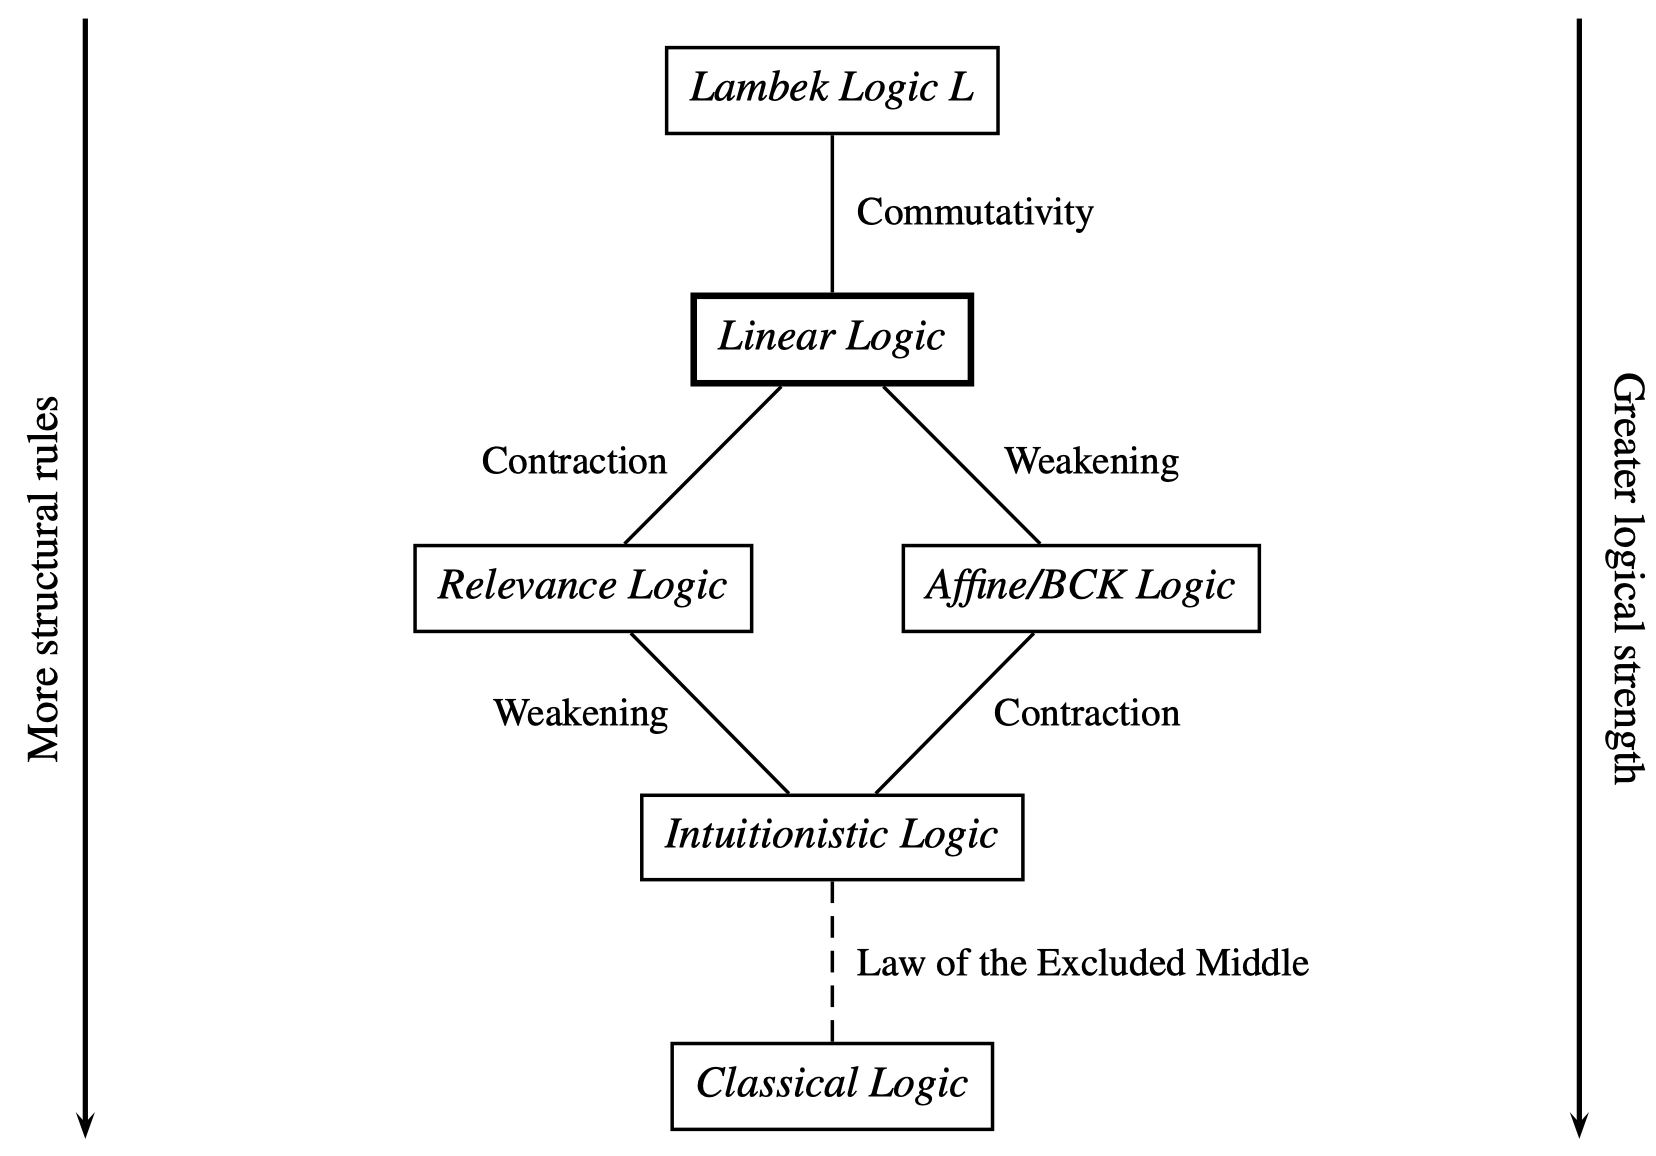
\includegraphics[scale=.4]{figures/Glue/substructural-logics.png}
  \caption{\label{fig:hierarchy}Hierarchy of logics related by
  structural rules  \citep[103; used with permission]{Asudeh12}}
  \label{fig:Glue:1}
\end{figure}

The appropriate resource logic for semantics alone is a commutative
resource logic. Semantic composition is resource-sensitive but does not show
evidence of order-sensitivity in its own
right \citep[ch.\,5]{Asudeh12}. Consider the general case of some
binary structure that is to be
interpreted. If one branch denotes a function and the other denotes an
argument, the function applies to the argument, whether the function is on the
left or right:
\eabox{
  \attop{\ensuremath{
   \Lsem \raisebox{2em}[1.5em][1.5em]{\begin{forest}
    [ [\textbf{function}] [\textbf{argument}]]
    \end{forest}}\Rsem
    ~~$=$~~
   \Lsem \raisebox{2em}[1.5em][1.5em]{\begin{forest}
    [ [\textbf{argument}] [\textbf{function}]]
    \end{forest}} \Rsem}}
}
%
For example, in English basic word order, the function that is the
denotation of a transitive verb takes its argument to the right, but
the resulting function that is the denotation of the VP takes its
argument to the left. 

It is not the \emph{order} of the function and argument that determines their
composition, but rather their semantic types \citep{klein;sag85}. This
is saliently exemplified by the rule of functional application in the
widely familiar system of \citet[44,~95]{heim1998semantics}. It is also
exemplified by  the equivalent interpretations of the forward and backward slash
rules of Combinatory Categorial Grammar (see,
e.g., \citealt[406]{steedman87} or \citealt[186]{steedman;baldridge11}).

But how is semantics resource-sensitive? The following quote from
\citet[172]{klein;sag85} illustrates:
\begin{quote} 
  Translation rules in Montague semantics have the property that the
  translation of each component of a complex expression occurs exactly
  once in the translation of the whole. \ldots\ That is to say, we do not want
  the set S [of semantic interpretations of a phrase] to contain all
  meaningful expressions of IL [Intensional Logic] which can be built
  up from the elements of S, but only those which use each element
  exactly once.
\end{quote}  
%
In other words, \citegen{montague73} translation rules are
resource-sensitive. However, this is merely coincidental as far as his
translation process is concerned. In their generalization of Montague's
system, \citet[174]{klein;sag85} need to define an operation of
\aterm{bounded closure}. This operation ensures that the meaning of
each element of semantic composition is indeed used ``exactly once.''

We can obtain this result in a more general way, if we adopt a resource
logic for semantic composition. This rests on the absence of the
structural rules of contraction and weakening. The lack of contraction
means that the number of occurrences of a premise matters, so a set of
linear logic premises is a \aterm{multiset} (sometimes called a
\aterm{bag}). The lack of weakening means that the bag must be emptied
in constructing a valid proof. In other words, it follows directly
from the absence of contraction and weakening that \dquote{each
  element} must be used \dquote{exactly once}.  
\citegen{klein;sag85} bounded closure is effectively an attempt
to capture the logical resource sensitivity of linear logic or L \citep[110--111]{Asudeh12}.

Logical resource sensitivity in turn forms the basis for linguistic
resource sensitivity \citep[ch.\,4]{Asudeh12}. This is achieved by
 placing a linguistically motivated goal condition on the \glue\
logic proof; for example, we can require that the proof of a sentence
terminates in a single meaning constructor of type \aterm{t}
\citep{dalrymple;ea99c}. \citet[110--123]{Asudeh12} argues that
resource-sensitive composition not only directly captures bounded
closure, it arguably also captures a diverse set of principles across
a variety of frameworks. These include Completeness and Coherence
\citep{kaplanbresnan82}, the Theta Criterion \citep{chomsky1981lectures}, the
Projection Principle \citep{chomsky1981lectures,chomsky1982some,chomsky86a}, No
Vacuous Quantification
\citep{chomsky1982some,chomsky1995the-minimalist,kratzer95,kennedy97,heim1998semantics,fox00},
the Principle of Full Interpretation \citep{chomsky86a,chomsky1995the-minimalist}, and
the Inclusiveness Condition \citep{chomsky1995the-minimalist}.

\largerpage
In addition, it seems that phonology and syntax can equally be
considered resource-sensitive, i.e.\ lack weakening and contraction
from a logical perspective, as outlined in
\citet[98--99]{Asudeh12}. This allows a deeper generalization
about natural language as computation \citep{steedman07}, namely that
\emph{natural language is resource-sensitive}. The claim is set out in
the \aterm{Resource Sensitivity Hypothesis}
\citep[95]{Asudeh12}. Where phonology and syntax contrast with
semantics is not with respect to weakening and contraction, but rather
with respect to commutativity. Phonology is strictly non-commutative,
whereas syntax shows commutativity in some circumstances of free word
order. This leaves two options. The partial commutativity of syntax
can be captured by separating the syntax of structure from the
syntax of composition, treating the syntactic module(s) autonomously, as in
\glues. Alternatively, partial commutativity can be captured by not
separating structural and compositional syntax  and instead  introducing a mechanism to the syntax--semantics
interface that relaxes commutativity in what is otherwise a
non-commutative system. An example of such a mechanism is the
categorial modalities of \citet{baldridge02}.

%\clearpage


\section{Glue without LFG: Flexible composition}
\label{sec:general-glue}

Linguistic meanings in \glue\ are encoded in \aterm{meaning
  constructors}. Meaning constructors are pairs of terms from two
logics. These terms can be represented as \formula{\mathcal{M}} and
\formula{G} (where \formula{\mathcal{M}} is mnemonic for \aterm{meaning
  language} and \formula{G} is mnemonic for \aterm{\glue\ logic}). These could be written in any conventional way for writing
pairs, such as \formula{\langle\mathcal{M},G\rangle}, but most Glue work of the past couple
of decades has written the pair using an uninterpreted colon as a
pairing symbol, as in (\ref{ex:Glue:8}):
\ea\label{ex:Glue:8}
\formula{\mathcal{M}:G}
\z
%
The meaning language can be anything that supports the lambda
calculus, such as the simply typed lambda calculus that is often used
in linguistic semantics. However, more specialized lambda languages
can be used, as in \citet{genabith;crouch99}, 
  \citet{bary;haug11}, and \citet{lowe15-sanskrit}, which all use
  \citegen{muskens96} Compositional Discourse Representation Theory
  (CDRT) or \citet[ch.\,14]{DLM:LFG}, which uses
  \citegen{Haug2014} partialized version, Partial Compositional
  DRT (PCDRT).  The glue logic is a fragment of \aterm{linear logic}
  \citep{girard1987}. The glue logic specifies semantic composition
  based on a syntactic parse that instantiates the general terms in
  \formula{G} to a specific syntactic structure. The meaning
  constructors thus serve as \aterm{premises} in a linear logic
  \aterm{proof} of the compositional semantics.


\largerpage
The 
linear logic implication connective, $\multimap$,\footnote{This is the
  \aterm{multimap} symbol, but it is often referred to 
  in Glue discourse as the \aterm{lollipop}.} is the basis for the
fundamental compositional rule of functional application. Functional
application corresponds to linear implication elimination 
in  natural deduction style:
\ea
\label{ex:implE} 
  \nohigh{Functional application:}
  \\
  \nohigh{Implication 
    elimination}
  \hfill \mbox{modus ponens}\\[1ex]
%   \\[1.5ex]
  \begin{tabular}[t]{c}
    \begin{prooftree}
      \formula{\beta:A \linimp B} \hspace*{2em} \formula{\alpha:A}
      \justifies
      \formula{\beta(\alpha):B} \using \linimpE
    \end{prooftree}
  \end{tabular}
\z\clearpage

\noindent
The implication elimination rule is standard modus ponens. The rule is
read as follows: given \formula{\beta:A \linimp B} and given \formula{\alpha:A}, it is valid to conclude  \formula{\beta(\alpha):B}. 

The Curry-Howard Isomorphism
\citep[CHI;][]{curry;feys58,howard80} determines the correspondence between the
term to the left of the colon --- a term from \formula{\mathcal{M}}
--- and the term to right of the colon --- a term from  \formula{G}.
The CHI puts logical
formulas in correspondence with computational types. Here linear logic
formulas are in correspondence with  types in the
lambda calculus.\footnote{Some early papers in \glue\
  \citep{dalrympleetal93,dalrymple;ea95b,dalrymple;ea97b,crouch;gena99,genabith;crouch99,Fry:99,kehler;ea99}
  used a more ad-hoc method of relating the meaning terms to the
  \glue\ logic, but \citet{dalrymple;ea97,dalrymple;ea99c} introduced
  the Curry-Howard approach to \glue, which is now standard. \citet{kokkonidis08} introduced an
  alternant called \aterm{First-Order \glue} which has also proven
  influential in subsequent \glue\ literature (e.g.,
  \citealt{bary;haug11}, \citealt{Lowe2014}, \citealt{gotham:minimalist-glue}, \citealt{gotham-haug:2018},
  \citealt{findlay2019}; see also \citealt{andrews10} for a related
  proposal).} The terms \formula{A,B} in \exrr{implE} are schematic for possibly
complex formulas; \formula{\alpha,\beta} may similarly be complex
terms.

The rule for linear implication introduction
corresponds to functional abstraction.
\ea
\label{ex:implI} 
  \nohigh{Functional abstraction:}
  \\*
  \nohigh{Implication introduction}
  \hfill \mbox{hypothetical reasoning}
  \\*[1.5ex] 
  \begin{tabular}[t]{c}
    \begin{prooftree}
      \[\formula{[\alpha:A]}^1 
        \leadsto
        \formula{\beta:B}\]
      \justifies
      \formula{\lambda \alpha.\beta:A \linimp B} \using \linimpIi{1}
    \end{prooftree}
  \end{tabular} 
\z
%
In this schema, a hypothesis
is uniquely flagged with a numerical index. The fact that it is a
hypothesis --- i.e.\ not a premise encoded by a meaning constructor --- is indicated by square brackets. If a conclusion can be derived through some series of
proof steps (indicated by the vertical ellipsis), given the
hypothesis, then we know that the hypothesis implies the conclusion: the hypothesis
is discharged (as the antecedent of an implication with the conclusion
as the consequent) and its flag is withdrawn. In the meaning language,
this
corresponds to abstraction over the variable introduced on the meaning
language 
side of the hypothesis.

Let's turn to a simple linguistic example:
\ea
Blake called Alex. 
\z
%
Let us assume the following meaning constructor for the verb
\word{called}, leaving tense aside:\footnote{\label{fn:eta}Note that the
  lambda term $\formula{\lambda
  y.\lambda x.\IT{call}(y)(x)}$ is equivalent to the function 
  \formula{\IT{call}} by 
  $\eta$-equivalence in the lambda calculus. However, it is useful for
 the exposition below 
  to present it in non $\eta$-reduced form.}
\ea \label{ex:semantics-1} 
\formula{\lambda
  y.\lambda x.\IT{call}(y)(x):a \linimp b \linimp c}
\z
%
On the \glue\ side, \formula{c} is mnemonic for \word{called},
\formula{a} for \word{Alex}, and \formula{b} for \word{Blake}. This
meaning constructor would in fact be specified in
some general form but instantiated relative to a particular syntactic
structure. For now, let us just assume that some instantiation has given us the
meaning constructor in (\ref{ex:semantics-1}). In \sectref{sec:glue-lfg} below,
we'll see how to specify meaning constructors in general terms given
LFG's usual f-description language. 

Assuming that the lexical entries for \word{Alex} and \word{Blake}
contribute meaning constructors that are instantiated to
\formula{\IT{alex}:a} and \formula{\IT{blake}:b}, we can construct
the following proof, given \exrr{semantics-1}; note that
$\Rightarrow_\beta$ indicates $\beta$-reduction of a lambda term. 
\eabox{
\label{ex:simple-proof} \attop{
    \begin{prooftree}
      \formula{\IT{blake}:b}
      \[
        \formula{\lambda
          y.\lambda x.\IT{call}(y)(x):a \linimp b \linimp c}
        \hspace*{2em}
        \formula{\IT{alex}:a}
        \justifies
        \formula{\lambda x.\IT{call}(\IT{alex})(x):b \linimp c}
        \using \linimpE, \Rightarrow_\beta
      \]
      \justifies
        \formula{\IT{call}(\IT{alex})(\IT{blake}):c}
        \using \linimpE, \Rightarrow_\beta
    \end{prooftree}
    }
}
%
The meaning term in the conclusion is equivalent to
\formula{\IT{call}(\IT{blake},\IT{alex})} in the commonly used
  relational notation \citep{montague73}. 

Note that proofs are abstract mathematical objects that can be
written down in various ways. This is quite apart from whatever convention
or notation we choose for writing them down. For example, even holding
constant our natural deduction notation, what is shown in
\exrr{simple-proof} is just one of four ways to write down the single
abstract normal form proof \citep{prawitz65}. Writing the proof down
imposes an order,\footnote{The \word{Alex} meaning constructor/premise must be
  written either to the right or left of the functional (verb) meaning constructor and similarly
  for the \word{Blake} meaning constructor/premise.} but since the \glue\ logic is commutative
(see \sectref{sec:glue-logic} for further details), all four
written representations of the proof are equivalent. 

Given the commutativity of the \glue\ logic, the arguments of the
function can be freely reordered (re-curried), as in \exrr{semantics-2}
below, but still yield the appropriate meaning:
\ea\label{ex:semantics-2}
  \formula{\lambda
  x.\lambda y.\IT{call}(y)(x):b \linimp a \linimp l}
\z
%
Example \exrr{semantics-3} below is a schematic demonstration of how this argument reordering
works in a proof; the example abstracts away from the particular \IT{call}
function. The example also shows the implication introduction rule in
action. 
\eabox{\label{ex:semantics-3}
  \attop{
    \begin{prooftree}
%      \[
      \[
      \[
      \[
        \[        
        \formula{\lambda y.\lambda x.f(y)(x):a \linimp b \linimp c}
        \hspace*{2em}
        \formula{[v:a]\textsuperscript{1}}
      \justifies
      \formula{\lambda x.f(v)(x):b \multimap c}
      \using
      \linimpE
      \]
      [u:b]\textsuperscript{2}
      \justifies
      \formula{f(v)(u):c}
      \using
      \linimpE
      \]
      \justifies
      \formula{\lambda v.f(v)(u):a \multimap c}
      \using
      \linimpIi{1}
    % \]
    % \justifies
    % \formula{\lambda y.f(y)(u):a \multimap c}
    % \using \Rightarrow_\alpha
  \]
  \justifies
    \formula{\lambda u.\lambda v.f(v)(u):b \multimap a \multimap c}
    \using
    \linimpIi{2}
  \]
  \justifies
  \formula{\lambda x.\lambda y.f(y)(x):b \multimap a \multimap c}
  \using \Rightarrow_\alpha, \Rightarrow_\alpha
\end{prooftree}
}
%\medskip\\
}

\noindent
The result is a reordered form of the original term but without any
change in meaning, because the CHI ensures that the function's
arguments in the  meaning terms are
also appropriately reordered.  The $\alpha$-equivalences, in which variables are
renamed, are not strictly
necessary, but have been added for full transparency. In general, given $n$ arguments in the order
\formula{a_1 \ldots a_n}, a reverse order \formula{a_n \ldots
  a_1} can be obtained by a series of hypotheses on the
arguments that are discharged in the order they were made. More
generally, the arguments can be reordered in any order by mixing the
order of hypothesis assumption and discharge. 


% More generally, given some head \formula{h} and some arguments of this head
% \formula{a_1, \ldots, a_n}, the implicational term associated with the
% head would be \formula{a_1 \linimp \ldots \linimp a_n \linimp h}.

\largerpage[-1]
\section{The syntax--semantics interface: Autonomy of syntax}
\label{sec:glue-interface}


\glue\ rests on two general  assumptions about the syntax--semantics
interface:
%
\begin{enumerate}
\item\label{item:2} \label{item:1} The \aterm{logical syntax} of semantic composition
  \citep{fenstad;ea87} is distinct from the \aterm{structural
    syntax}. The syntax of linear logic proofs captures the logical
  syntax in \glue. Some separate syntactic framework, such as LFG,
  captures the structural syntax of categorially determined
  distribution, constituency, features, and local and non-local
  dependencies (i.e, \aterm{syntax} in the standard sense).
\item\label{item:3} Logical syntax and structural syntax are systematically related 
  through the instantiation of \glue\ meaning constructors. 
\end{enumerate}
%
These assumptions distinguish \glue\ from both \aterm{interpretive
  theories} of semantic composition and \aterm{parallel theories} of
semantic composition. A well-known example of interpretive theories is
Logical Form semantics \citep[e.g.,][]{heim1998semantics}. The \aterm{description-by-analysis}
semantics for LFG of \citet{halvorsen83} is another example of an
interpretive theory. Two well-known examples of parallel theories are
Combinatory Categorial Grammar \citep[e.g.,][]{steedman;baldridge11}
and Type-Logical Categorial Grammar
\citep[e.g.,][]{carpenter97}.\footnote{Parallel theories are often
  discussed under the rubric of \dquote{rule-by-rule composition}
  \citep{bach:extension}, but the \aterm{rule-by-rule} 
  term is no longer accurate. The term originates in the paired
  syntactic/semantic rules of \citet{montague73}, which is now
  deprecated. This kind of theory is also sometimes
  referred to as \dquote{direct compositionality}
  \citep{barker;jacobson07,jacobson14}, but this raises a number of
  issues \citep{asudeh2006direct}, so I do not favour that term.}

With respect to LF semantics, 
\glue's assumption of a separate level of structural syntax is similar. However, in its standard co-descriptive guise, \glue\
is distinct from LF semantics, because \glue\ does not assume that the
syntactic structure in its entirety is the input to semantic
interpretation. With respect to Categorial Grammar, we also see
similarity and divergence. We see similarity in \glue's assumption
of the pairing of functional application (the fundamental
compositional operation) with terms that define complex categories
implicationally.\footnote{Categorial Grammar's slashes are directed
  implications. 
  For example, X{\fs}Y states
  that one can conclude a category X conditional on there being a
  category Y to the right; in other words, X{\fs}Y means that Y $\rightarrow$ X yields X
  so long as Y is on the right of X.} However, \glue\ is also distinct from
Categorial Grammar, because \glue\ does not assume that implicational
categories are responsible for word order (hence their lack of
directionality), but rather that there is a separate syntactic
representation. In sum, \glue\ is a compositional semantic theory of a
third kind. From a big picture perspective, \glue\ synthesizes certain
aspects of LF semantics and Categorial Grammar, yet remains distinct
from both these theories. 

\largerpage[-2]
The assumptions, in \ref{item:2} and \ref{item:3} above, that began this section 
derive a strong notion of syntactic autonomy. Categorial Grammar makes
the very strong assumption that syntax and semantics are
isomorphic. This assumption entails that any semantic distinction must
be the reflection of  a syntactic
distinction. LF semantics similarly assumes that any
interpretive/semantic distinction 
must be due to an underlying syntactic distinction. In an
interpretive semantic theory such as LF semantics, the needs
of semantics dictate what's in the syntax, even if the things in
question are syntactically questionable. The predicate abstraction/numerical nodes in
\citet[186]{heim1998semantics} are an example, since they require the
addition of lambda operators to the syntactic tree. This is surprising
from the perspective of semantic theory, since this means that 
\emph{object} languages, i.e. the natural languages undergoing
analysis, must in fact contain these logical operators, for which
there is no compelling evidence (such as lexicalization in some
language or other). 

\newpage
Quantifier scope ambiguity offers perhaps the most straightforward
demonstration of the distinction between \glue\, on the one hand, and
LF semantics and Categorial Grammar, on the other. Consider the
following standard example:
\ea
\label{ex:scope} Everybody loves somebody. 
\z
%
The \glue\ logic computes two readings for this sentence, but
\emph{without} imputing a syntactic ambiguity, which seems
structurally under-motivated; see \S~\ref{sec:quantifier-scope} for
further details. This contrasts
with both LF semantics and Categorial Grammar; these theories both require the
two readings to be {syntactically} distinguished. 

In the next section, I pair \glue\ with LFG as the syntactic framework
in order to render these general points more
specific. Although LFG is the natural syntactic framework to choose,
given the present venue and the fact that most \glue\ work has assumed
an LFG syntax, see 
\sectref{sec:intro} above for a list of other syntactic
frameworks that have been paired with \glue.

\section{\glue\ with  LFG: Syntax/semantics non-isomorphism}
\label{sec:glue-lfg} 

% XX
% Pairing \glue\ with LFG, \lfgglue, also allows us to
% demonstrate flexible composition, as well as syntax/semantics
% non-isomorphism.

Consider the example in
\figref{fig:finn-eng1}, which shows the c-structures and
f-structure for the sentence \word{I drank water} in Finnish and
English.\footnote{I assume LFG's theory of \aterm{extended heads},
  which allows the Finnish verb to be generated in I
  \citep[ch.\,6--7]{BresnanEtAl2016,BresnanEtAl2016}.}  The distinct 
c-structures capture the variation in syntactic realization between
the two languages. In particular, they capture the fact that Finnish allows null subjects,
unlike English. The f-structure shows that these
distinct c-structures encode identical syntactic features and
dependencies. \figref{fig:finn-eng2}
shows the same structures with the arrows resolved. One way to solve
the equations is to label all c-structure nodes that bear a down arrow
with an f-structure variable. Instantiation of the metavariables
$\uparrow$ % \up\
and $\downarrow$ is arbitrary, barring accidental identity, and
resolves the equalities \citep[54--58]{BresnanEtAl2016}. 

\begin{figure}
  \centering
  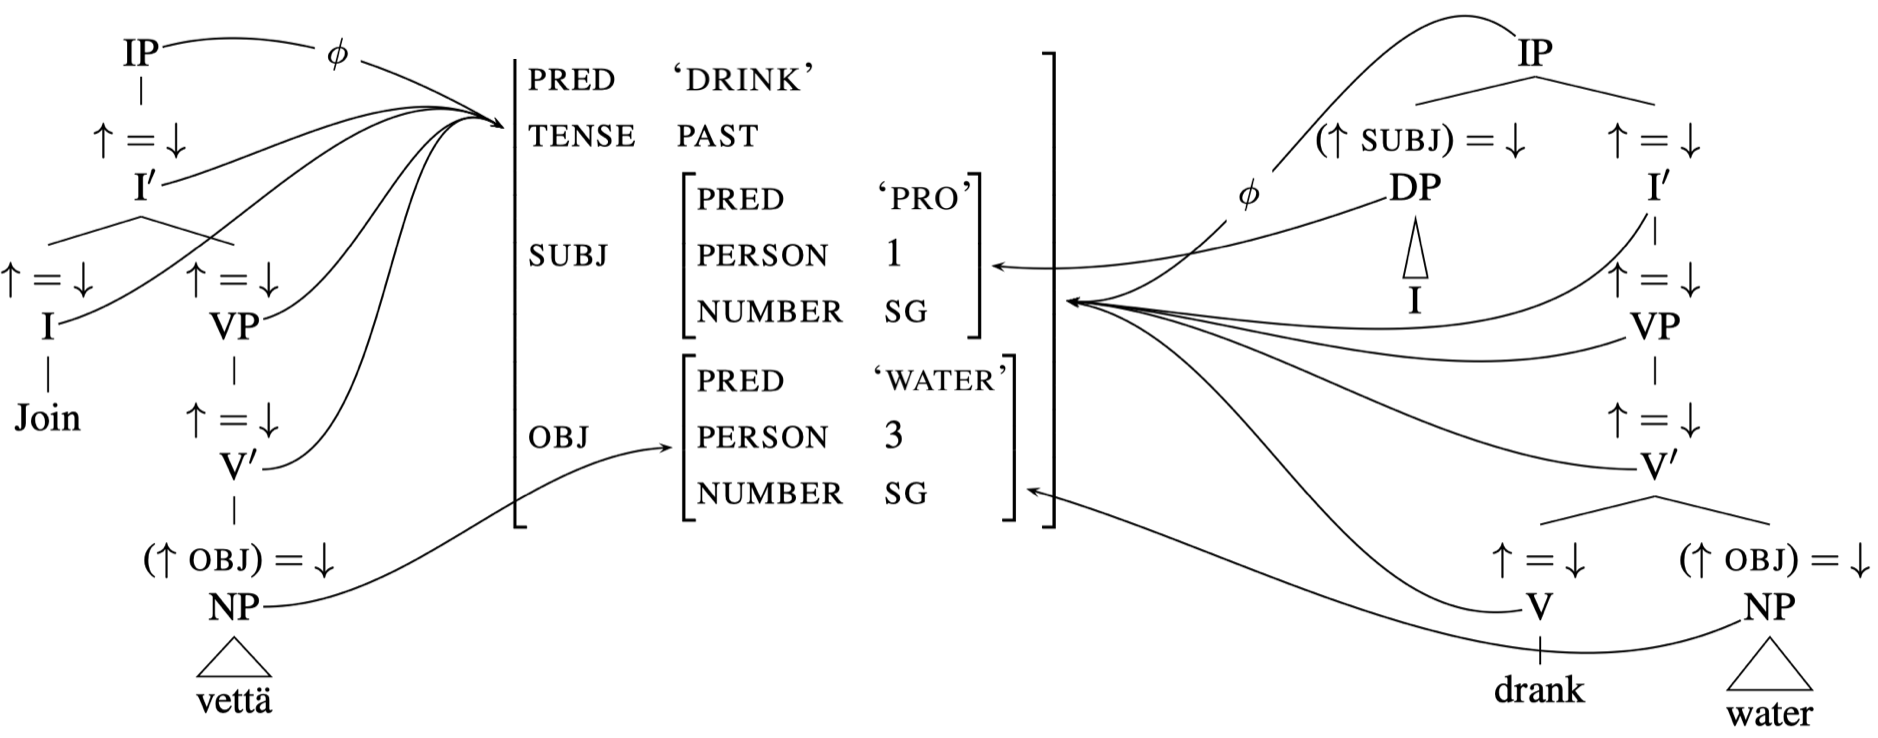
\includegraphics[scale=.32]{figures/Glue/finnish-english-1.png}
  \caption{C-structures and f-structure for \word{I drank water} in 
    Finnish and English (adapted from
    \citealt[27]{asudeh;toivonen15-lfg}; used with permission)}
  \label{fig:finn-eng1} 
\end{figure}

\begin{figure}
  \centering
  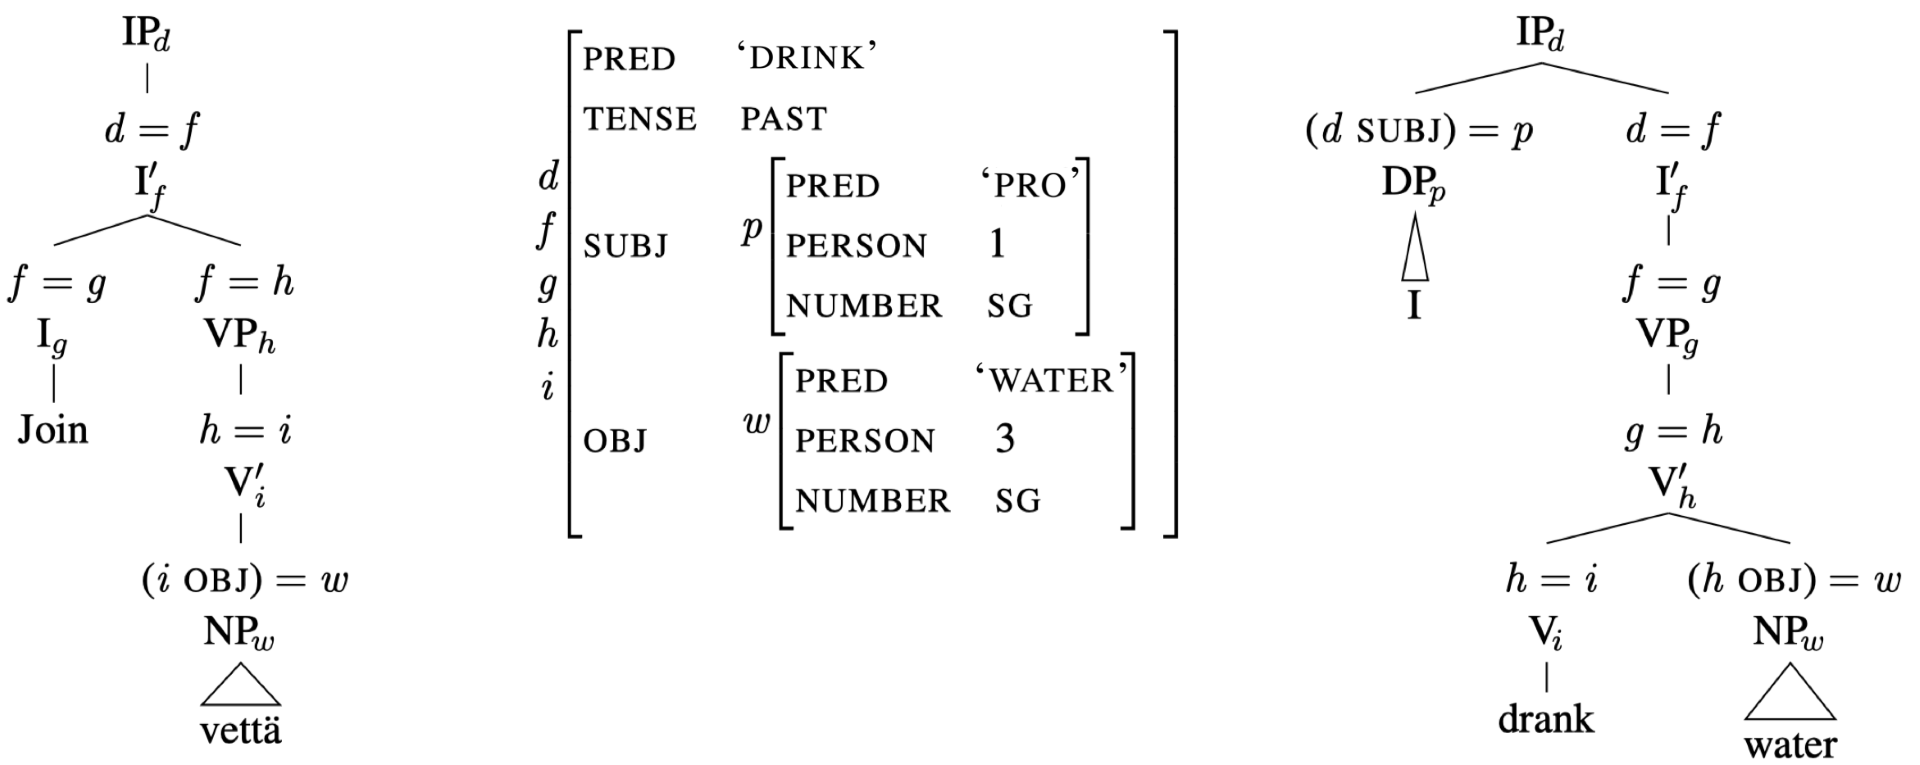
\includegraphics[scale=.33]{figures/Glue/finnish-english-2.png}
  \caption{Finnish and English structures with $\uparrow$ and $\downarrow$
    metavariables resolved (\citealt[330]{asudeh22}; used with permission)}
  \label{fig:finn-eng2} 
\end{figure}

In both the Finnish and English c-structures, the mapping to \feat{object} is contributed structurally by the annotation (\UP\OBJ) $=$ \Down\ on the NP daughter of {V$'$}. In the English c-structure, the
mapping to \feat{subject} is also contributed
structurally, by the annotation (\UP\SUBJ) $=$ \Down\ on the DP in SpecIP. In contrast, the
\feat{subject} information is contributed morphologically in the
Finnish c-structure. This distinction is reflected in the lexical
entries in \tabref{tab:lexicons}. Notice that the
f-descriptions in these lexical entries not only describe their
lexical contributions to f-structure, but also have appropriate \glue\ meaning constructors that define the mappings
to s(emantic)-structure and encode the composition of the head and its
dependents as linear implications.\footnote{The asterisk in the
  term for \word{vett\"{a}}/\word{water} is the cumulativity operator
  of \citet{link83}. It states that \IT{water} is a mass term,
  although this is not important for our present purposes.} I have
set tense aside in the semantics, but return to it in
\sectref{sec:tense} below.   The annotation $\sigma$ on
the arrows in the \glue\ meaning constructors indicates that these are the
s-structure correspondents of the relevant f-structures. The
$\sigma$ correspondence function maps from f-structure to
s-structure.

\begin{table}
  \tabcolsep7.5pt
%\centering
\smallskip
\scalebox{.85}{
\begin{tabular}{@{}l|l@{}}
\hline
  Finnish & English\\
  \hline\\[-1.5ex]
  \begin{tabular}[t]{@{}rcl@{}}
    \word{join} & I &
                       \begin{tabular}[t]{{@{}lcl@{}}}
                         (\UP \PRED) $=$ \pred{`drink'}\\
                         (\UP\TENSE) $=$ \val{past}\\
                         (\UP\SUBJ\PRED) $=$
                         \pred{`pro'}\\
                         (\UP\SUBJ\PERS) $=$ \val{1}\\
                         (\UP\SUBJ\NUM) $=$ \val{sg}\\[1ex]
                         \formula{\IT{speaker}:(\UP~\SUBJ)\sigb}\\[.5ex]
                         \formula{\IT{drink}:}\\
                         \formula{(\UP~\OBJ)\sig
                         \linimp (\UP~\SUBJ)\sig \linimp \upsigb}
                       \end{tabular}

    \\ \\
  
    \word{vett\"{a}} & N &
                       \begin{tabular}[t]{{@{}lcl@{}}}
                         (\UP \PRED) $=$ \pred{`water'}\\
                         (\UP\PERS) $=$ \val{3}\\
                         (\UP\NUM) $=$ \val{sg}\\[1ex]
                         \formula{\IT{*water}:\upsig}
                       \end{tabular}
  \end{tabular}
  
  &

  \begin{tabular}[t]{@{}rcl@{}}
    \word{I} & D & 
                       \begin{tabular}[t]{{@{}lcl@{}}}
                         (\UP \PRED) $=$ \pred{`pro'}\\
                         (\UP\PERS) $=$ \val{1}\\
                         (\UP\NUM) $=$ \val{sg}\\[1ex]
                         \formula{\IT{speaker}:\upsigb}
                       \end{tabular}

    \\ \\
    
    \word{drank} & V &
                       \begin{tabular}[t]{{@{}lcl@{}}}
                         (\UP \PRED) $=$ \pred{`drink'}\\
                         (\UP\TENSE) $=$ \val{past}\\[1ex]
                         \formula{\IT{drink}:}\\
                         \formula{(\UP~\OBJ)\sig
                         \linimp (\UP~\SUBJ)\sig \linimp \upsigb}
                       \end{tabular}

    \\ \\

    \word{water} & N &
                       \begin{tabular}[t]{{@{}lcl@{}}}
                         (\UP \PRED) $=$ \pred{`water'}\\
                         (\UP\PERS) $=$ \val{3}\\
                         (\UP\NUM) $=$ \val{sg}\\[1ex]
                         \formula{\IT{*water}:\upsig}
                       \end{tabular}
\vspace*{1.5ex}
  \end{tabular}
  \\  
  \hline
\end{tabular}
}
\caption{Lexicons for \word{I drank water} in Finnish and English}
\label{tab:lexicons}
\end{table}



The up arrows in \tabref{tab:lexicons} are instantiated to the
f-structure of the relevant pre-terminal node: \fsa{g} (Finnish
\word{join}), \fsa{w} (Finnish \word{vett\"{a}}), \fsa{p} (English
\word{I}), \fsa{i} (English \word{drank}), and \fsa{w} (English
\word{water}).\footnote{In the case of the abbreviated (triangle)
  structures, there would be intervening nodes. But there would be a
  chain of \updown\ annotations between the word and the phrase it
  heads, so this is a harmless simplification.} However, we know
from \figref{fig:finn-eng2} that \fsa{g}\;$=$\;\fsa{i}\;$=$\;\fsa{d}. So we can just use the mnemonic label \fsa{d} in all relevant
cases. We
can also take advantage of the equality (\fsa{d} \feat{subj}) $=$
\fsa{p}. We obtain the 
following collection of identical instantiated meaning constructors
for each language:% \footnote{Note that $\Gamma$ is a multiset, not a
  % set, due to the \glue\ logic's lack of contraction, and that the
  % only valid proof empties this multiset, due to the \glue\ logic's
  % lack of weakening; see \sectref{sec:glue-logic} above.}
\ea
\{\formula{\IT{speaker}:p\sigb},
  \formula{\IT{drink}:w\sig \linimp p\sig \linimp d\sigb}, \formula{\IT{*water}:w\sigb}\}
\z
%
This yields a single normal form proof (i.e., minimal proof;
\citealt{prawitz65}) for the corresponding Finnish and English
sentences, which can be presented in natural deduction format as
follows (recall that order of premises on a proof line does not
matter, since the \glue\ logic is commutative):
\eabox{
%  \textit{Proof}\\
  \attop{
    \begin{prooftree}
    \formula{\IT{speaker}:p\sigb}
    \[
      \formula{\IT{drink}:w\sig \linimp p\sig \linimp d\sigb}
      \hspace*{2em}
      \formula{\IT{*water}:w\sigb}
      \justifies
      \formula{\IT{drink}(\IT{*water}):p\sig \linimp d\sigb}
      \using \linimpE
    \]
    \justifies
    \formula{\IT{drink}(\IT{*water})(\IT{speaker}):d\sigb}
    \using \linimpE
  \end{prooftree}
  }
}
%
% This concludes the demonstration of the basics of \glue\ at the syntax--semantics
% interface, using LFG as the syntactic framework.

%\section{Analyses in \glues: Some representative cases}

\section{Some applications of glue semantics}


\subsection{Quantifier scope}
\label{sec:quantifier-scope}

Let us return to the quantifier scope example in \exrr{scope}
above, repeated here as \exrr{scope2}. 
\ea\label{ex:scope2}  Everybody loves somebody. 
\z
%
\glue's properties of autonomy of syntax
and  flexible composition allow \exrr{scope2} to be treated as 
\emph{syntactically unambiguous} but 
\emph{semantically ambiguous}.

I will not show the c-structure here, as  the relevant syntactic
representation is the single f-structure for \exrr{scope2} shown here, with mnemonic
labels as usual:
\ea
\label{ex:scope-fs}
\evnup{\avm[style=fstr]{\id{l}{[pred & {`love'}\\
             tense & pres \\
             subj & \id{e}{[pred & {`everybody'}\\
                            person & 3\\ 
                            number & sg]\vspace*{1ex}}\\
             obj & \id{s}{[pred & {`somebody'}\\
                            person & 3\\ 
                            number & sg]}]}}
                      }
\z        
% 
The \glue\ meaning constructors in the lexical entries are shown in
\exrr{scope-lex}. Tense has again been set aside and it is again most
transparent for expository purposes to show the meaning term for
\word{loves} in non-$\eta$-reduced form (see footnote~\ref{fn:eta} on $\eta$-reduction).
\ea
\label{ex:scope-lex}
   \begin{tabular}[t]{@{}rcl@{}}
    \word{everybody} & D & 
                           \begin{tabular}[t]{{@{}lcl@{}}}
                             \formula{\lambda Q.\IT{every}(\IT{person},Q):\forall S.(\upsig
                             \linimp\ S) \linimp\ S} 
                           \end{tabular}
   % \end{tabular}

   %  \medskip

   %  \begin{tabular}[t]{@{}lcl@{}}
\\[.5ex]
                           
   \word{somebody} & D & 
                       \begin{tabular}[t]{{@{}lcl@{}}}
                         \formula{\lambda Q.\IT{some}(\IT{person},Q):\forall S.(\upsig
                         \linimp\ S) \linimp\ S}
                       \end{tabular}
  %  \end{tabular}

  %   \medskip

  % \begin{tabular}[t]{@{}lcl@{}}
 \\[.5ex]
                          
  \word{loves} & V &
                       \begin{tabular}[t]{{@{}lcl@{}}}
                         \formula{\lambda y.\lambda x.\IT{love}(y)(x):(\UP~\OBJ)\sig
                         \linimp (\UP~\SUBJ)\sig \linimp \upsigb}
                       \end{tabular}
  \end{tabular}
\z
%
When we instantiate the meaning constructors in \exrr{scope-lex} relative to the f-structure in \exrr{scope-fs}, we get:
\ea \label{ex:scope-premises} $\Gamma$ $=$
  \begin{tabular}[t]{@{}l@{}}
    \{\,\formula{\lambda y.\lambda x.\IT{love}(y)(x):s
    \linimp\ e \linimp\ l},\\
    \phantom{\{}\,\formula{\lambda
    Q.\IT{every}(\IT{person},Q):\forall S.(e \linimp\ S) \linimp\
    S},\\
    \phantom{\{}\,\formula{\lambda
    Q.\IT{some}(\IT{person},Q):\forall S.(s \linimp\ S) \linimp\ 
    S}\,\}
  \end{tabular}
\z
%
\begin{sloppypar}
  \noindent The functions \IT{every} and \IT{some} are standard quantificational
  determiners from generalized quantifier theory
  \citep{montague73,barwise;cooper81,keenan;faltz85}, with type
  \bracket{\bracket{e,t},\bracket{\bracket{e,t},t}}. The function
  \IT{every} is defined
  as \formula{\lambda P.\lambda Q.P \subseteq Q}. The function
  \IT{some} is defined as 
  \formula{\lambda P.\lambda Q.P \cap Q \neq \varnothing}. In these formulas, 
  \formula{P} is the set of entities that is the determiner's
  restriction and \formula{Q} is the set of entities that is its
  scope.  The quantifier \formula{\lambda
    Q.\IT{every}(\IT{person},Q)} thus returns true if the set
  of people is a subset of its scope set. Similarly, the quantifier
  \formula{\lambda Q.\IT{some}(\IT{person},Q)} returns true if the
  intersection of the set of people and its scope set is non-empty.
\end{sloppypar}

A comment is in order about 
the universal quantification symbol $\forall$ in the \glue\ 
terms for the quantifiers. This universal ranges over variables in the \glue\ logic. It
allows the quantifier scope over \emph{any}  \glue\ logic
  dependency on the semantic correspondent of the quantifier. 
\citet[393--394]{Asudeh05reln} discusses the
interpretation of $\forall$ in linear logic. The
key insight is that, given the resource sensitivity of linear
logic, the universal means \dquote{any one}, not
\dquote{all}. The function of the linear universal is to define \aterm{scope
  points} and its interpretation is not related to the
quantificational force in the meaning language. Observe that \IT{every} and
\IT{some} alike are   associated with these linear universal
scope terms, even though \IT{some} has existential force.

\hspace*{-5.5pt}The meaning constructors in \exrr{scope-premises} yield exactly two
normal form/minimal proofs. These can be represented as in
\figref{fig:surf-scope} and~\figref{fig:inv-scope}.\footnote{The
  universal linear instantiation step is trivial, as in
  classical/intuitionistic logic. I have therefore not shown it
  explicitly. See \citet[396]{Asudeh12} for the rule.} In other
theories, quantifier scope ambiguity requires either a syntactic operation such as
Quantifier Raising (QR) in Logical Form semantics
\citep{may77,may85,heim1998semantics} or a type shifting operation and corresponding categorial
modification of some kind, as in
Combinatory or Type-Logical Categorial Grammar semantics
\citep{partee;rooth83,hendriks93}. Thus, interpretive and parallel
theories of composition alike impute a syntactic ambiguity to handle
quantifier scope ambiguity.\footnote{\citet[ch.\,14]{jacobson14} offers a
  textbook comparison of the LF and CG approaches.}

This contrasts with \glues. 
The fact that \glue\ assumes an independent level of syntax (autonomy
of syntax) allows composition to be flexible (flexible composition),
which in turn allows the theory to derive the two distinct scope
readings without positing a syntactic ambiguity or type shift.

\begin{figure}
  \centering
  \scalebox{0.76}{
    \begin{prooftree}
      \formula{\lambda Q.\IT{every}(\IT{person},Q):\\\forall S.(e
        \multimap S) \multimap S}
      \[
        \[
          \formula{\lambda Q.\IT{some}(\IT{person},Q):\\\forall
            S.(s \multimap S) \multimap S}
          \[
            \[
              \[
                \formula{\lambda y.\lambda x.\IT{love}(y)(x):\\s
                  \multimap e \multimap l} \hspace*{2em} \formula{\
                  \\{}[v:s]^1} \justifies \formula{\lambda
                  x.\IT{love}(v)(x):\\e \multimap l} \using
                \linimpE, \Rightarrow_\beta
              \]
              \formula{\ \\{}[u:e]^2} \justifies
              \formula{\IT{love}(v)(u):l} \using \linimpE,
              \Rightarrow_\beta
            \]
            \justifies \formula{\lambda y.\IT{love}(y)(u):\\s
              \linimp l} \using \linimpIi{1}, \Rightarrow_\alpha
          \]
          \justifies \formula{\IT{some}(\IT{person},\lambda
            y.\IT{love}(y)(u)):l} \using \linimpE,
          \forallE [l/S], \Rightarrow_\beta
        \]
        \justifies \formula{\lambda
          x.\IT{some}(\IT{person},\lambda
          y.\IT{love}(y)(x)):\\e \linimp l} \using \linimpIi{2},
        \Rightarrow_\alpha
      \]
      \justifies \formula{\IT{every}(\IT{person},\lambda
        x.\IT{some}(\IT{person},\lambda y.\IT{love}(y)(x))):l}
      \using \linimpE, \forall_{\mathcal{E}} [l/S], \Rightarrow_\beta
    \end{prooftree}
  }
  \bigskip
  \caption{Surface scope interpretation of
    \word{Everybody loves somebody}}
  \label{fig:surf-scope}
\end{figure}

%\clearpage

\begin{figure}
  \centering
  \scalebox{.76}{
    \begin{prooftree}
      \formula{\lambda Q.\IT{some}(\IT{person},Q):\\\forall S.(s
        \multimap S) \multimap S}
      \[
        \[
          \formula{\lambda Q.\IT{every}(\IT{person},Q):\\\forall
            S.(e \multimap S) \multimap S}
              \[
                \formula{\lambda y.\lambda x.\IT{love}(y)(x):\\s
                  \multimap e \multimap l} \hspace*{2em} \formula{\
                  \\{}[v:s]^1} \justifies \formula{\lambda
                  x.\IT{love}(v)(x):\\e \multimap l} \using
                \linimpE, \Rightarrow_\beta
              \]
          \justifies \formula{\IT{every}(\IT{person},\lambda
            x.\IT{love}(v)(x)):l} \using \linimpE,
          \forall_{\mathcal{E}} [l/S], \Rightarrow_\beta
        \]
        \justifies \formula{\lambda
          y.\IT{every}(\IT{person},\lambda
          x.\IT{love}(y)(x)):\\s \linimp l} \using \linimpIi{1},
        \Rightarrow_\alpha
      \]
      \justifies \formula{\IT{some}(\IT{person},\lambda
        y.\IT{every}(\IT{person},\lambda x.\IT{love}(y)(x))):l}
      \using \linimpE, \forall_{\mathcal{E}} [l/S], \Rightarrow_\beta
    \end{prooftree}
  }
  \bigskip
  \caption{Inverse scope interpretation of \word{Everybody loves somebody}}
  \label{fig:inv-scope}
\end{figure}




\subsection{Modification}
\label{sec:modification}

\glue\ is similar to Categorial Grammar in offering an analysis of
semantic \aterm{modification} such that modifiers are easily
identifiable by their formal shape. For example, the nominal
modification category in \exrr{cg-mod} has its \glue\ logic analog in
\exrr{glue-mod} (leaving the meaning language aside):
\ea\label{ex:cg-mod} N\fs N
\ex \label{ex:glue-mod} \formula{A_{\langle e,t\rangle} \linimp
    A_{\langle e,t \rangle}}
\z
%
\begin{sloppypar}
  \noindent A nominal modifier is a functional category/type that takes a
  nominal category/type as an input and returns the same category/type
  as an output. The modificational semantics is captured on the
  meaning language side.
\end{sloppypar}

For example, a \glue\ meaning constructor for the attributive
adjective \word{Finnish} would look like \exrr{glue-mod-finnish}.
\ea\label{ex:glue-mod-finnish} \formula{\lambda P\lambda x.P(x)
    \wedge \IT{finnish}(x):(a_e \linimp b_t) \linimp (a_e \linimp b_t)}
\z
%
Continuing the example, the common noun \word{city} would provide the
\bracket{e,t} input to
the main implication in \exrr{glue-mod-finnish}, such that
\word{Finnish city} would correspond to the following (composed)
result:
\ea \formula{\lambda x.\IT{city}(x)
    \wedge \IT{finnish}(x):(a_e \linimp b_t)}
\z
%
More generally, a modifier of any type corresponds to a meaning
constructor with the following form:
\ea \label{ex:glue-mod-gen} \formula{\lambda f.\IT{mod}(f):X
    \linimp X}\z
%
The function \IT{mod} is a placeholder for whatever the semantic
effect of the modifier is.

The property of syntax-semantics non-isomorphism, which allows a
lexical item to contribute multiple meaning constructors, allows a
natural and elegant analysis of so-called \aterm{recursive
  modification} \citep{kasper97}. In a nominal like the following, the
result we want is that it is apparently the case that the city in question
is Finnish:
\ea
apparently Finnish city
\z
%
In other words, we somehow want to maintain a consistent semantics for
\word{apparently} as a modifier, while nevertheless
allowing it to fulfill this modificational role inside a nominal. This
is despite the type clash between the modifier,
which expects a proposition-forming type as input, and the 
adjective \word{Finnish}, which does not have this type. The adjective
instead 
has the type of a modifier, i.e. a function on the type that
the interpretation of \word{apparently} expects. 

The solution in \glue\ is to associate predicative and attributive adjectives with
the property denotation for the adjective, shown in the first line of
\exrr{glue-mod-rec}, and to further add a general nominal
modification meaning constructor to the lexical entry for the
attributive adjective, as in the second line of \exrr{glue-mod-rec}.
\ea \label{ex:finnish-adj-lex}\label{ex:glue-mod-rec} \lexentry{Finnish}{\formula{\lambda
      x.\IT{finnish}(x):v \linimp f}\\
  (~~\formula{\lambda Q\lambda P\lambda x.Q(x) \wedge P(x):(v \linimp f)
    \linimp (a \linimp b) \linimp (a \linimp b)}~~) }
\z
%
The reader can verify that the combination of these two meaning
constructors yields the meaning constructor in \exrr{glue-mod-finnish} above (with
types omitted). The second meaning constructor is treated as optional
to ensure that predicative uses of the adjective work as
expected. Resource-sensitive composition ensures that a predicative
occurrence of the adjective cannot use the second meaning constructor whereas
an attributive occurence must use it. 

The revised analysis allows recursive modification by a
modifier like \word{apparently}, assuming that we have a meaning
constructor like the following associated with \word{apparently},
suitably instantiated to an f-structure where \word{apparently} is in
the \feat{adj} set of \word{finnish}:
\ea \label{ex:glue-apparently} \lexentry{apparently}{\formula{\lambda
    P\lambda x.\IT{apparently}(P(x)):(v \linimp f) \linimp (v
    \linimp f)}}
\z
%
The combination of this meaning constructor for \word{apparently} and
the first meaning constructor in \exrr{finnish-adj-lex} then yields
the following:
\ea \label{ex:app-finn} \formula{\lambda x.\IT{apparently}(\IT{finnish}(x)):v \linimp f}
\z
%
This is sufficient for a predicative occurrence, as in \word{Marimekko 
  is apparently Finnish}.

For attributive occurrences, \exrr{app-finn} then combines with the
second meaning constructor in \exrr{finnish-adj-lex}, which yields the
desired result:
\ea \formula{\lambda P\lambda x.\IT{apparently}(\IT{finnish}(x)) \wedge
    P(x):(a \linimp b) \linimp (a \linimp b)}
\z
%
This would then combine with the interpretation of \word{city} 
to yield the correct interpretation for, e.g., \word{The apparently
  Finnish city is nice}.

I leave aside here the natural extension that is necessary to fully
capture recursive modification in examples like the following:
\ea apparently obviously Finnish 
\z
%
The extension just involves having two separate meaning constructors
for the adverbial modifier \word{obviously} (and \word{apparently},
etc.), in order to make the system fully general, much as we have for the adjective \word{Finnish} in
\exrr{finnish-adj-lex}.

The first proposal for the extended modificational semantics presented
here was in \citet[255--274]{dalrymple01}, to my knowledge. The most recent version
of the \lfgglue\ approach to modification, including recursive
modification, is the subject matter of \citet[ch.\,13]{DLM:LFG}. 

\subsection{Tense}
\label{sec:tense}

The basic approach to modification that was sketched at the beginning
of Section \ref{sec:modification} supports a simple account of tense
as a modifier on a basic verb meaning, provided that we add a tense
coordinate to verb meanings \citep[for a review of approaches to tense
in compositional semantics, see][]{gronn;stechow16}.

Let us assume that a basic meaning constructor for a verb now looks like this:
\ea \label{ex:sigh-tense} \lexentry{sigh}{\formula{\lambda x\lambda
      t.\IT{sigh}(t,x):\textup{\textit{subj}} \linimp \textup{\textit{tense}} \linimp verb}}
\z
%
Let's also assume, following \cite{haug08}, that \formula{u} stands
for utterance time (what \citealt{gronn;stechow16} denote as
\formula{s^*}, for speech time). Then we can capture simple present,
past and future tense as follows, with the \glue\ logic instantiated
suitably per the terms in \exrr{sigh-tense}:\footnote{These sorts of
  meanings assume a model of time as consisting of points, but it may
  well be preferable to think of time as consisting of intervals
  \citep{Dowty1979}. An interval-based semantics poses no problem for
  tense in \glues\ per se, but I've chosen to keep things simple here.}
\ea
\label{ex:tense-mcs}
  \ea
\lexentry{\textsc{\textup{past}}}{\formula{\lambda P\lambda t.P(t) \wedge
      t \prec u:(\textup{\textit{tense}} \linimp verb) \linimp (\textup{\textit{tense}} \linimp verb)}} 
\ex \lexentry{\textsc{\textup{present}}}{\formula{\lambda P\lambda t.P(t) \wedge
      t = u:(\textup{\textit{tense}} \linimp verb) \linimp (\textup{\textit{tense}} \linimp verb)}}  
\ex \lexentry{\textsc{\textup{future}}}{\formula{\lambda P\lambda t.P(t) \wedge
      u \prec t:(\textup{\textit{tense}} \linimp verb) \linimp (\textup{\textit{tense}} \linimp verb)}}
  \z
\z
% 
This sort of account is obviously too simple, but it illustrates tense
as a modifier. Note that I've presented the tenses ``on their own''
for maximal perspicuity, but in a lexicalist framework such as LFG,
one would normally assume that tense-inflected forms are inserted in
the syntax as words, formed morpholexically. That would just mean
that, for example, the inflected form \word{sighed} would contribute
both the meaning constructor in \exrr{sigh-tense} and the one in
\exrr[a]{tense-mcs}. Note also that I assume some kind of suitable
eventual existential closure of the temporal variable. 

One could also incorporate grammatical (as opposed to lexical) aspect
in a similar, modificational manner. For analyses of tense and
grammatical aspect in \glues, see \citet{haug08}, \citet{bary;haug11},
and \citet{Lowe2014,lowe15-sanskrit}.\footnote{Some of this work assumes some version
  of event 
  semantics (sketched in
  \sectref{sec:events}). However, event semantics is
  not necessary for a basic treatment of tense, as I've illustrated
  here.}

\subsection{Events}
\label{sec:events}

The first \glue\ analysis to incorporate event semantics
\citep{davidson67,parsons1990events,champollion17}  
was never published \citep{fry99,fry05}. To my knowledge, the first
major publications to use event semantics were
\citet{AshT:12} and \citet{asudeh2013constructions}. Much like
the analysis of tense sketched above, event semantics for \glue\
involves adding a dependency on an event variable. Moreover, work in
event semantics in \glue\ has generally taken the Neo-Davidsonian
approach of \citet{parsons1990events}, in which verbs (and other
predicates that take event-arguments) denote functions from events to truth
values, such that the arguments of the verb are actually modifiers of
the event variable. For example, the sentences in
\exrr{events-act-pass} would receive an interpretation like
\exrr{events-act-pass-int}, whereas the sentence in
\exrr{events-short-passive} would receive an interpretation like
\exrr{events-short-passive-int}.\footnote{It is also possible to treat
verbs as generalized quantifiers over events \citep{champollion17,coppock;champollion20}, but I'm not
aware of any \glue\ work thus far that has taken this tack and it
wouldn't make a difference to the sorts of simple cases sketched here.}
\ea
\label{ex:events-act-pass}
  \ea Sam hugged Max.
  \ex Max was hugged by Sam.
  \z 
\ex \label{ex:events-act-pass-int} \formula{\exists e.\IT{hug}(e) \wedge \IT{agent}(e) =
    \IT{sam} \wedge \IT{patient}(e) = \IT{max}}
\ex \label{ex:events-short-passive} Max was hugged.
\ex \label{ex:events-short-passive-int} \formula{\exists e\exists
    x.\IT{hug}(e) \wedge \IT{agent}(e) =
    x \wedge \IT{patient}(e) = \IT{max}} 
\z
%
It can be observed from \exrr{events-act-pass-int} and
\exrr{events-short-passive-int} that the event variable is eventually
existentially closed. This is a standard assumption in event
semantics. 

\begin{sloppypar}
  Event semantics is a natural meaning language for \glues,
  because the event variable permits a highly factorized semantics,
  using LFG's \aterm{template} language \citep{dalrymple2004linguistic}, which
  is designed to allow generalizations to be captured across
  grammatical elements, including meaning constructors. This in turn
  maximizes the analytic leverage offered by flexible composition and
  syntax/semantics non-isomorphism.
\end{sloppypar}

For example, the lexical entry for the verb \word{hugged} (again
leaving tense aside) can capture
its underlying semantic bivalence by encoding a dependency on a
\feat{subject} and \feat{object} (as well as the event
variable):\footnote{It has been common in Glue work on event
  semantics to use \formula{e,e',e''}, etc., as variables over events,
  but a common convention in event semantics more generally is to use
  \formula{v,v',v''}, etc.\ \citep[e.g.,][]{champollion17,coppock;champollion20}.}
\ea
\label{ex:hug-lex} \lexentry{hugged}{\formula{\lambda y\lambda x\lambda
      e.\IT{hug}(e) \wedge \IT{agent}(e) = x \wedge
      \IT{patient}(e) = y:\\
      \gterm{obj} \linimp \gterm{subj} \linimp \gterm{event} \linimp \gterm{verb}
    }
    }
\z
%
We can take advantage of pervasive syncretism in the English passive
participle here and assume that the meaning constructor in
\exrr{hug-lex} is associated with the past tense and passive
participle alike.

We can then treat the passive voice as contributing a modificational meaning
constructor that remaps the arguments, as in \exrr{passive-lex}. I
again associate this with an abstract formative to gloss over details
of lexicalization \citep[for a related proposal,
see][185--186]{findlay2019}.\footnote{Note that the treatment
  sketched here uses mnemonics for f-structure grammatical functions,
  like \textit{subj}, in the Glue terms. However, actual Glue work in
  this vein uses Glue terms defined with respect to argument
  structure, as sketched in the next section. See
  \citet[75--76]{AsudGior12} and \citet[77ff.]{asudeh2014meaning} for further details.}
\ea
\label{ex:passive-lex} \lexentry{\textsc{\textup{passive}}}{
    \formula{\lambda P\lambda x\lambda y.P(x)(y):
      \formula{(\gterm{obj} \linimp \gterm{subj} \linimp \gterm{verb}) \linimp \\
      \gterm{subj} \linimp \gterm{obl} \linimp \gterm{verb}
      }}
  }
\z
%
Note that this entry requires implication elimination on the
\formula{\gterm{event}} term in the verb's meaning constructor and
then reintroduction of the term (for eventual existential binding of
the corresponding variable) after the passive modifier has composed
with the verb's meaning constructor. We will shortly add a second
meaning constructor to the entry for \textsc{passive}, but this one
suffices to capture the truth-conditional equivalence of
\exrr[a--b]{events-act-pass} (which is not to say that they are
information-structurally equivalent).

The result of combining the meaning constructor in \exrr{passive-lex}
with the one in \exrr{hug-lex} is passive \word{hugged}: 
\ea \label{ex:hug-lex-pass} \lexentry{hugged\textsc{\textup{+passive}}}{\formula{\lambda x\lambda y\lambda
      e.\IT{hug}(e) \wedge \IT{agent}(e) = y \wedge
      \IT{patient}(e) = x:\\
      \gterm{subj} \linimp \gterm{obl} \linimp \gterm{event} \linimp \gterm{verb}
    }
    }
  \z
  %
  In other words, the passive voice modifies the meaning of
  \word{hugged} such that the passive subject corresponds to the
  logical object (the patient in this case) and passive
  \word{by}-phrase corresponds to the logical subject (the agent in
  this case).\footnote{I have implicitly assumed in my choice of
    mnemonic, \formula{obl}, that the \word{by}-phrase is an
    \feat{oblique}, but nothing hinges on this. The same term works if
    it is treated as an \feat{adjunct}, although its mnemonic function
    is obscured.} \figref{fig:hug-passive} shows the proof for
  \exrr[b]{events-act-pass}. The reader can verify that the result is
  the same interpretation as that of \exrr[a]{events-act-pass}. The
  interpretation for \exrr[a,b]{events-act-pass} is shown in
  \exrr{events-act-pass-int} above.

\begin{sloppypar}
  But what of the short passive in \exrr{events-short-passive}? Here
  we can leverage optionality and the properties of resource-sensitive
  composition and syntax/semantics non-isomorphism to naturally extend
  the analysis. We simply add an optional meaning constructor to
  \exrr{passive-lex}, such that the revised lexical entry is as
  follows:
\end{sloppypar}
\ea
\label{ex:passive-lex2} \lexentry{\textsc{\textup{passive}}}{
    \formula{\lambda P\lambda y\lambda x.P(x)(y):
      \formula{(\gterm{obj} \linimp \gterm{subj} \linimp \gterm{verb}) \linimp \\
      \gterm{subj} \linimp \gterm{obl} \linimp \gterm{verb})}
    }\\[3ex]
    (~~\formula{\lambda P\exists x.P(x):(\gterm{obl} \linimp
      \gterm{verb}) \linimp \gterm{verb}}~~)
  }
\z
%
The optional entry allows the passive to also contribute a second
meaning constructor that existentially binds the subject argument. If
there is an actual subject resource, though, as in the long passive in
\exrr[b]{events-act-pass}, resource sensitivity ensures that the
optional meaning constructor cannot be used, because then the actual
subject resource would go unused. \figref{fig:hug-short-passive} shows
  the proof for \exrr[b]{events-act-pass}. The reader can verify that
  the result is the same interpretation as that of
  \exrr{events-short-passive}, shown in
  \exrr{events-short-passive-int} above. 

The use of event semantics in \lfgglue\ has become especially common
in a thread of work on argument structure, the topic that we turn to
next.

%\clearpage

%
\begin{figure}[tbp]
  \centering
  \scalebox{0.6}{
    \hspace*{5.25em}
    \begin{prooftree}
      \[
      \[
      \[
        \vformula{by Sam}{\IT{sam}:\\obl}
        \hspace*{-0em}
        \[
          \vformula{Max}{\IT{max}:\\subj}
                  \hspace*{-14em}
      \[
      \[
        \[
      \[
      \[
      \[
        \[
          \[
            \[
              \vformula{hugged}{ \lambda y\lambda x\lambda
                e.\IT{hug}(e) \wedge \IT{agent}(e) = x \wedge
                \IT{patient}(e) = y:\\
                \gterm{obj} \linimp \gterm{subj} \linimp \gterm{event}
                \linimp \gterm{verb} } \vformula{}{\ \\{}[u:obj]^1}
              \justifies \formula{\lambda x\lambda e.\IT{hug}(e)
                \wedge \IT{agent}(e) = x \wedge
                \IT{patient}(e) = u:\\
                \gterm{subj} \linimp \gterm{event} \linimp
                \gterm{verb}}
    \using \linimpE 
            \]
            \formula{\ \\{}[v:subj]^2} \justifies \formula{\lambda
              e.\IT{hug}(e) \wedge \IT{agent}(e) = v \wedge
              \IT{patient}(e) = u:\gterm{event} \linimp \gterm{verb}}
    \using \linimpE 
          \]
          \formula{[e':event]^3} \justifies \formula{\IT{hug}(e')
            \wedge \IT{agent}(e') = v \wedge 
            \IT{patient}(e') = u:\gterm{verb}}
    \using \linimpE 
        \]
        \justifies
        \formula{\lambda v.\IT{hug}(e') \wedge
          \IT{agent}(e') = v \wedge \IT{patient}(e') =
          u:\gterm{subj} \linimp \gterm{verb}}
        \using \linimpIi{2}
      \]
      \justifies \formula{\lambda u\lambda v.\IT{hug}(e')
        \wedge \\ \IT{agent}(e') = v \wedge \IT{patient}(e') =
        u:\\\gterm{obj} \linimp \gterm{subj} \linimp \gterm{verb}} \using
      \linimpIi{1}
    \]
    \vformula{\feat{\textup{passive}}}{
      \lambda P\lambda x\lambda y.P(x)(y):\\
      (\gterm{obj} \linimp \gterm{subj} \linimp \gterm{verb}) \linimp \\
      \gterm{subj} \linimp \gterm{obl} \linimp \gterm{verb}
      }
    \justifies
    \formula{
      (\lambda P\lambda x\lambda y.P(x)(y))(\lambda u\lambda v.\IT{hug}(e')
      \wedge \IT{agent}(e') = v \wedge \IT{patient}(e') =
      u):\gterm{subj} \linimp \gterm{obl} \linimp \gterm{verb}
    }
    \using \linimpE 
  \]
  \justifies
  \formula{
      \lambda x\lambda y.(\lambda u\lambda v.\IT{hug}(e')
      \wedge \IT{agent}(e') = v \wedge \IT{patient}(e') =
      u)(x)(y):\gterm{subj} \linimp \gterm{obl} \linimp \gterm{verb}
    }
    \using \Rightarrow_\beta
  \]
  \justifies
   \formula{
      \lambda x\lambda y.(\lambda v\lambda e'.\IT{hug}(e')
      \wedge \IT{agent}(e') = v \wedge \IT{patient}(e') =
      x)(y):\gterm{subj} \linimp \gterm{obl} \linimp \gterm{verb}
    }
    \using \Rightarrow_\beta
  \]
  \justifies
   \formula{
      \lambda x\lambda y\lambda e'.\IT{hug}(e')
      \wedge \IT{agent}(e') = y \wedge \IT{patient}(e') =
      x:\\\gterm{subj} \linimp \gterm{obl} \linimp \gterm{verb}
    }
    \using \Rightarrow_\beta
  \]
  \justifies
   \formula{
     \lambda y.\IT{hug}(e')
      \wedge \IT{agent}(e') = y \wedge \IT{patient}(e') =
      \IT{max}:\\\gterm{obl} \linimp \gterm{verb}
    }
    \using \linimpE 
  \]  
  \justifies
   \formula{
     \IT{hug}(e')
      \wedge \IT{agent}(e') = \IT{sam} \wedge \IT{patient}(e') =
      \IT{max}:\gterm{verb}
    }
    \using \linimpE 
  \]
  \justifies
  \formula{
     \lambda e'.\IT{hug}(e')
      \wedge \IT{agent}(e') = \IT{sam} \wedge \IT{patient}(e') =
      \IT{max}:\gterm{event} \linimp \gterm{verb}
    }
    \using \linimpIi{3}
  \]
  \justifies
  \formula{
     \lambda e.\IT{hug}(e)
      \wedge \IT{agent}(e) = \IT{sam} \wedge \IT{patient}(e) =
      \IT{max}:\gterm{event} \linimp \gterm{verb}
    }
    \using \Rightarrow_\alpha
  \]
  \justifies
  \formula{
     \exists e.\IT{hug}(e)
      \wedge \IT{agent}(e) = \IT{sam} \wedge \IT{patient}(e) =
      \IT{max}:\gterm{verb}
    }
    \using \exists_\textit{event}
    \end{prooftree}
  }
\caption{Proof for passive \exrr[b]{events-act-pass}, \textit{Max was
    hugged by Sam}}
 % showing combination of meaning constructor for
 %  \word{hugged} with meaning constructor for \feat{passive}
\label{fig:hug-passive}
\end{figure}
%
\begin{figure}[tbp]  \centering
  \scalebox{0.5875}{
    \begin{prooftree}
      \[
      \[
      \[
      \[
      \[
        \vformula{\feat{passive}}{\lambda P\exists x.P(x):\\(\gterm{obl} \linimp
      \gterm{verb}) \linimp \gterm{verb}}
        \hspace*{-0em}
        \[
          \vformula{Max}{\IT{max}:\\subj}
                  \hspace*{-13em}
      \[
      \[
        \[
      \[
      \[
      \[
        \[
          \[
            \[
              \vformula{hugged}{ \lambda y\lambda x\lambda
                e.\IT{hug}(e) \wedge \IT{agent}(e) = x \wedge
                \IT{patient}(e) = y:\\
                \gterm{obj} \linimp \gterm{subj} \linimp \gterm{event}
                \linimp \gterm{verb} } \vformula{}{\ \\{}[u:obj]^1}
              \justifies \formula{\lambda x\lambda e.\IT{hug}(e)
                \wedge \IT{agent}(e) = x \wedge
                \IT{patient}(e) = u:\\
                \gterm{subj} \linimp \gterm{event} \linimp
                \gterm{verb}}
              \using \linimpE 
            \]
            \formula{\ \\{}[v:subj]^2}
            \justifies
            \formula{\lambda
              e.\IT{hug}(e) \wedge \IT{agent}(e) = v \wedge
              \IT{patient}(e) = u:\gterm{event} \linimp \gterm{verb}}
              \using \linimpE 
          \]
          \formula{[e':event]^3}
          \justifies \formula{\IT{hug}(e') \wedge \IT{agent}(e') = v \wedge
            \IT{patient}(e') = u:\gterm{verb}}
              \using \linimpE 
        \]
        \justifies
        \formula{\lambda v.\IT{hug}(e') \wedge
          \IT{agent}(e') = v \wedge \IT{patient}(e') =
          u:\gterm{subj} \linimp \gterm{verb}}
        \using \linimpIi{2}
      \]
      \justifies
      \formula{\lambda u\lambda v.\IT{hug}(e')
        \wedge \\ \IT{agent}(e') = v \wedge \IT{patient}(e') =
        u:\\\gterm{obj} \linimp \gterm{subj} \linimp \gterm{verb}}
      \using
      \linimpIi{1}
    \]
    \vformula{\feat{\textup{passive}}}{
      \lambda P\lambda x\lambda y.P(x)(y):\\
      (\gterm{obj} \linimp \gterm{subj} \linimp \gterm{verb}) \linimp \\
      \gterm{subj} \linimp \gterm{obl} \linimp \gterm{verb}
      }
    \justifies
    \formula{
      (\lambda P\lambda x\lambda y.P(x)(y))(\lambda u\lambda v.\IT{hug}(e')
      \wedge \IT{agent}(e') = v \wedge \IT{patient}(e') =
      u):\gterm{subj} \linimp \gterm{obl} \linimp \gterm{verb}
    }
              \using \linimpE 
  \]
  \justifies
  \formula{
      \lambda x\lambda y.(\lambda u\lambda v.\IT{hug}(e')
      \wedge \IT{agent}(e') = v \wedge \IT{patient}(e') =
      u)(x)(y):\gterm{subj} \linimp \gterm{obl} \linimp \gterm{verb}
    }
    \using \Rightarrow_\beta
  \]
  \justifies
   \formula{
      \lambda x\lambda y.(\lambda v\lambda e'.\IT{hug}(e')
      \wedge \IT{agent}(e') = v \wedge \IT{patient}(e') =
      x)(y):\gterm{subj} \linimp \gterm{obl} \linimp \gterm{verb}
    }
    \using \Rightarrow_\beta
  \]
  \justifies
   \formula{
      \lambda x\lambda y\lambda e'.\IT{hug}(e')
      \wedge \IT{agent}(e') = y \wedge \IT{patient}(e') =
      x:\\\gterm{subj} \linimp \gterm{obl} \linimp \gterm{verb}
    }
    \using \Rightarrow_\beta
  \]
  \justifies
   \formula{
     \lambda y.\IT{hug}(e')
      \wedge \IT{agent}(e') = y \wedge \IT{patient}(e') =
      \IT{max}:\\\gterm{obl} \linimp \gterm{verb}
    }
              \using \linimpE 
  \]  
  \justifies
   \formula{
     (\lambda P\exists x.P(x))(\lambda y.\IT{hug}(e')
      \wedge \IT{agent}(e') = y \wedge \IT{patient}(e') =
      \IT{max}):\gterm{verb}          
    }
    \using \linimpE 
  \]
  \justifies
  \formula{
     \exists x.(\lambda y.\IT{hug}(e')
      \wedge \IT{agent}(e') = y \wedge \IT{patient}(e') =
      \IT{max})(x):\gterm{verb}
    }
  \using \Rightarrow_\beta
  \]
  \justifies
  \formula{
     \exists x.\IT{hug}(e')
      \wedge \IT{agent}(e') = x \wedge \IT{patient}(e') =
      \IT{max}:\gterm{verb}
    }
    \using \Rightarrow_\beta
  \]
  \justifies
  \formula{
     \lambda e'\exists x.\IT{hug}(e')
      \wedge \IT{agent}(e') = x \wedge \IT{patient}(e') =
      \IT{max}:\gterm{event} \linimp \gterm{verb}
    }
    \using \linimpIi{3}
  \]
  \justifies
  \formula{
     \lambda e\exists x.\IT{hug}(e)
      \wedge \IT{agent}(e) = x \wedge \IT{patient}(e) =
      \IT{max}:\gterm{event} \linimp \gterm{verb}
    }
    \using \Rightarrow_\alpha
    \]
    \justifies
  \formula{
     \exists e\exists x.\IT{hug}(e)
      \wedge \IT{agent}(e) = x \wedge \IT{patient}(e) =
      \IT{max}:\gterm{event} \linimp \gterm{verb}
    }
    \using \exists_\textit{event}
  \end{prooftree}
  }
\caption{Proof for short passive \exrr{events-short-passive}, \textit{Max was
    hugged}}
\label{fig:hug-short-passive}
\end{figure}


\subsection{Argument structure}

% \psnode{1}{hello}

% \psnode{2}{world} \rtor{2}{1}

There is a prominent strand of work in \glues\ on argument structure
and mapping theory (i.e., the realization of underlying arguments in
the syntax). Representative work in this vein includes
\citet{arnold;sadler12}, 
\citet{AsudGior12}, \citet{asudeh2014meaning}, \citet{asudeh:unrealized},
\citet{findlay14-mphil,findlay2017mapping,Findlay2020},
\citet{Lowe2015,lowe19-cp}, \citet{lowe;birahimani19},
\citet{Przep17a}, and \citet{Lovestrand2020}.

However, before turning to the \glue\ approach to argument structure, it is
worth presenting some of the background that led to it, because it
highlights another issue in \glues\ that has concerned some
researchers. The substance of the worry can be straightforwardly
summarized: What are the identity conditions for empty semantic
structures? In other words, if a semantic structure is an attribute
value matrix of some kind, as assumed from quite early on in the
development of \glues\ \citep{dalrymple;ea99c,dalrymple01}, how can
there be \emph{distinct} empty s-structures, since an empty AVM seems
to correspond to the empty set, which is unique \citep{kokkonidis08,findlay2021}? 
\eabox{
\label{ex:s-structure1}
  \attop{%
  \begin{tabular}[t]{lcl}
    \begin{tabular}[c]{l}
      \rnode[tr]{cf}{
      \avm[style=fstr]{
      \id{c}{[pred\hspace*{.75em} & {`call'}\\
      subj & \id{b}{[pred &
                                {`Blake'}]}\raisebox{.75ex}{\rnode{bf}{}}
                                \vspace*{.25em}
      \\
      obj & \id{a}{[pred & {`Alex'}]}\raisebox{.5ex}{\rnode{af}{}}]}
                               }}
    \end{tabular}
                              &\hspace*{2em}&
                                              \begin{tabular}[c]{l}
                                                \rnode[cl]{cs}{$c_\sigma$\avm[style=fstr]{[\\]}}\\\\
                                                \rnode[cl]{bs}{$b_\sigma$\avm[style=fstr]{[\\]}}\\\\
                                                \rnode[cl]{as}{$a_\sigma$\avm[style=fstr]{[\\]}}\\
                                              \end{tabular}
  \end{tabular}
}
  \nccurve[nodesepA=-1pt,nodesepB=1pt,angleA=42,angleB=180,linewidth=0.5pt]{->}{cf}{cs}
  \ncput*[npos=0.66]{$\sigma$}
  \nccurve[nodesepA=-1pt,nodesepB=1pt,angleA=42,angleB=180,linewidth=0.5pt]{->}{bf}{bs}
  \ncput*[npos=0.66]{$\sigma$}
  \nccurve[nodesepA=-1pt,nodesepB=1pt,angleA=42,angleB=180,linewidth=0.5pt]{->}{af}{as}
  \ncput*[npos=0.66]{$\sigma$}
}
% 
One possible solution to the empty s-structure problem is to make the
labelling part of the definition of the structure. In other words, if
a standard attribute-value  matrix is a finite set of attribute-value
pairs \citep[see, e.g.,][44]{BresnanEtAl2016}, then let us define an
s-structure as a finite set of pairs, where the first member of each
pair is a string (a unique label) and the second member of each pair
is a (possibly empty) AVM. In that case, it's clear that the
s-structure \{$\langle a_\sigma, \varnothing \rangle$\} does not equal the
s-structure \{$\langle b_\sigma, \varnothing \rangle$\}, even if both of them
have the empty AVM as their second coordinate. 

However, another issue with the sort of s-structure in
\exrr{s-structure1} is that it's really not a structure at all, since
the parts are not connected. In other words, what we have in
\exrr{s-structure1} is really \emph{three} s-structures, not a single
one. This does not make a substantive difference to the kinds of
proofs one can do in \glues, but it is a bit strange from a general
LFG-theoretic perspective, as we would expect all the modules in the
Correspondence Architecture to be structures and all of the ones that
have been proposed, aside from the version of s-structure above,
indeed are structures.

\citet{AsudGior12} solve this last problem by offering a
connected s-structure that also fulfills the role of
a(rgument)-structure \citep{butt1997architecture} in the Correspondence
Architecture. Not only does this eliminate the need for a-structure as
a separate module in the architecture, it also relates argument
structure and mapping theory more strongly to compositional semantics,
as the locus for both is now s-structure. \figref{fig:ag-as} shows the
\citet{AsudGior12} analysis for \exrr{eat-intrans}.
\ea
\label{ex:eat-intrans} Kim ate at noon. 
\z
%
The verb \word{ate} is semantically bivalent, since it entails that
there is something that has been eaten, but it can nevertheless be
syntactically intransitive \citep[71]{AsudGior12}. This is
reflected in the analysis in \figref{fig:ag-as}. There is no
\feat{object} in the f-structure, but there are two arguments in the
connected s-structure, which also serves as a representation of
argument structure.  

\begin{figure}
  \centering
  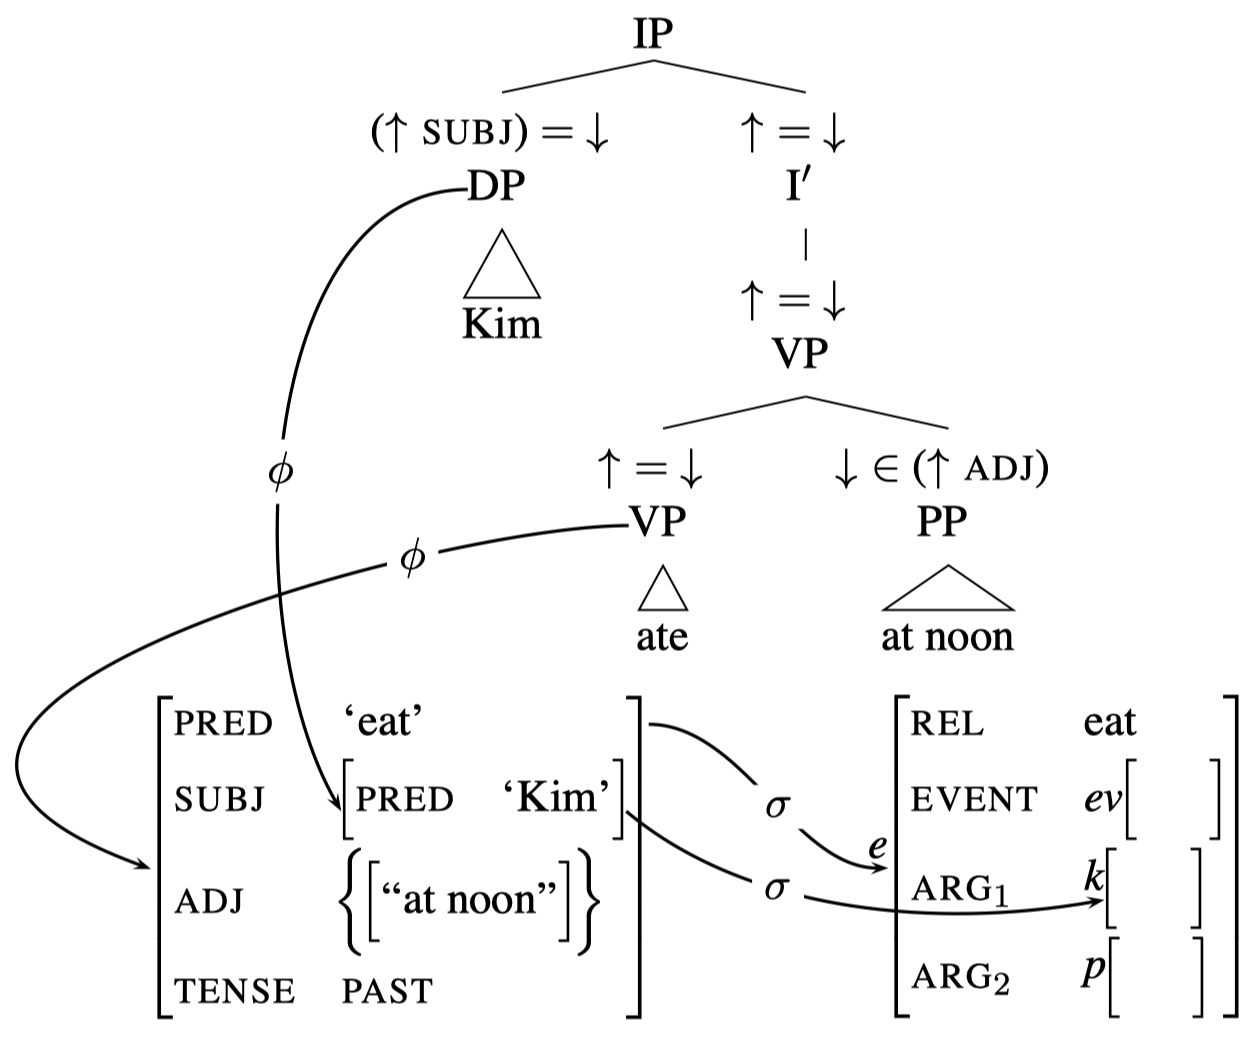
\includegraphics[scale=.4]{figures/Glue/arg-struc1.png}
  \caption{\label{fig:ag-as}\word{Kim ate at noon}  \citep[72; used with permission]{AsudGior12}}
\end{figure}

The solution to the syntax/semantics mismatch for the verb \word{ate}
is to allow the verb itself to contribute an optional second meaning
constructor that existentially closes the dependency on the second
argument:\footnote{Intransitive uses of semantically bivalent verbs
  also trigger presuppositions about the implicit argument \citep{fillmore86};
  e.g., \word{Kim ate at noon} presupposes that what Kim ate is food
  (for Kim). I do not attempt to model this here, but see
  \citet{AsudGior12} and \citet{asudeh:unrealized} for some further discussion.}
\ea \lexentry{ate}{
    \formula{\lambda y\lambda x\lambda e.\IT{eat}(e) \wedge
      \IT{agent}(e) = x \wedge \IT{patient}(e)=y:\\ \gterm{obj}
      \linimp \gterm{subj} \linimp \gterm{event} \linimp \gterm{verb}}\\[3ex]
    (~~\formula{\lambda P\exists x.P(x):(\gterm{obj} \linimp
      \gterm{verb}) \linimp \gterm{verb}}~~)
  }
\z
%
This treatment is similar to the one for the passive in
\exrr{passive-lex2}. Note that this is a simplification of the actual
approach in \citet{AsudGior12} and
\citet{asudeh2014meaning}, because in those approaches the \glue\ logic
terms are defined using \feat{arg} features at s-structure,
which allows the analysis to more naturally interact properly with argument
alternations. 


\subsection{Multiword expressions}
\label{sec:mwe}

Multiword expressions (MWEs) are a challenge to a lexicalist theory
like LFG, because they show a mixture of idiomaticity and productivity
in both their syntax and semantics \citep[ch.\,1]{findlay2019}. On the
one hand, we find expressions like \word{by and large} which are
idiosyncratic in both their syntax (apparently a coordination of a
preposition and an adjective) and semantics (the expression means
something similar to the adverb \word{mostly}, but this can't be
compositionally obtained from the usual meanings of its parts). On the other
hand, we find expressions like \word{spill the beans}, which are
syntactically unexceptional and possibly yield to a kind of
transpositional semantic analysis in which \sem{\word{spill}} $=$
\sem{\word{reveal}} and \sem{\word{the beans}} $=$ \sem{\word{the
    secret}}. Nevertheless, even with this MWE we see evidence of
particular syntactic and semantic restrictions. For example, the
object is necessarily the definite plural \word{beans} and other forms
are either excluded entirely (e.g., \#\word{a bean} or \#\word{the
  peas}) or else seem at best like metalinguistic word-play (e.g.,
\word{the legumes}).

In short, MWEs are challenging because they are
like words in the sense that they seem to be lexically stored
expressions but are like phrases in having syntactic parts and, in
some cases, these parts seem to be visible to syntactic
operations. For example, in
\word{It's too late: the beans have already been spilled}, the MWE has
been passivized and one part is modified by an adverbial. For a
lexicalist theory, simultaneously capturing these lexical and
non-lexical properties of MWEs is difficult. Indeed, in order to
account for this mixture of lexical and syntactic properties,
\citet{findlay2019} replaces the c-structural part of standard LFG
with Tree-Adjoining Grammar \citep[TAG;][]{joshi-etal1975,abeille-rambow2000book}, which allows expressions to be
associated with trees in the lexicon, rather than with a simple
category. TAG allows these trees to then be inserted or adjoined in
the phrasal syntax. \citet{findlay2019} calls the resulting
theory \aterm{Lexicalised LFG}, in a nod to Lexicalized TAG \citep{schabes-etal1988},
because it allows lexicalization of syntactic structures as TAG
trees while maintaining LFG's standard separate level of f-structure and a mapping
between the TAG-based c-structures and the f-structures. 

No matter how one captures the syntax of MWEs, the syntax/semantics
non-isomorphism of \glues\ naturally captures their syntax/semantics
mismatches and idiomaticity. For example, \figref{fig:by-and-large}
shows \citegen{findlay2019} \emph{lexical} entry for \word{by
  and large}. It is an adjunct tree, since this is a modifier. The
meaning of \word{by-and-large} is captured by the call to a template,
\feat{@By-And-Large-Meaning}, but we can simplify things as in
\exrr{by-and-large}.
\ea
\label{ex:by-and-large} \lexentry{by and large}{\formula{\lambda
    P\lambda x.\IT{mostly}(P(x)):(\gterm{subj} \linimp verb) \linimp (\gterm{subj} \linimp verb)}}
\z
%
This is a relatively straightforward example. For more complex
examples, see \citet{findlay2019}.

\begin{figure}
  \centering
  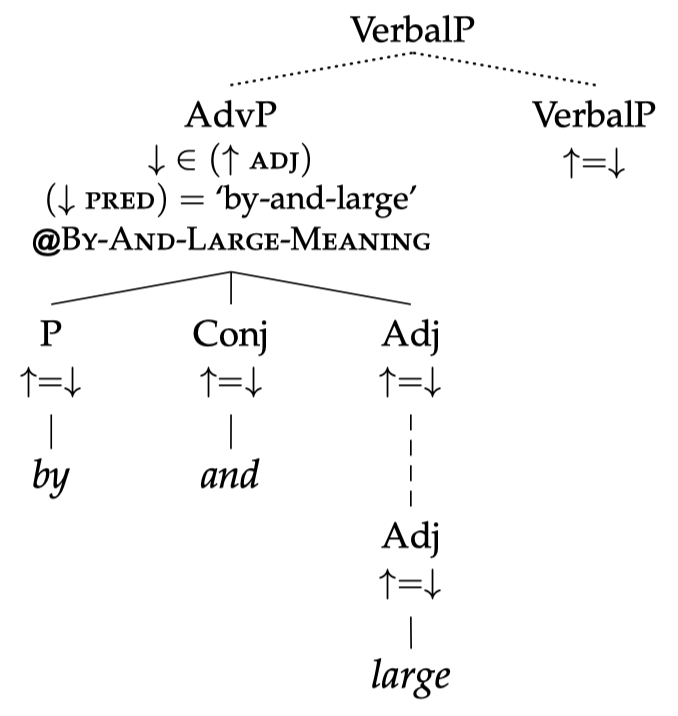
\includegraphics[scale=.5]{figures/Glue/by-and-large.png}
  \caption{\label{fig:by-and-large} Lexical entry for \word{by and large}   \citep[265; used with permission]{findlay2019}}
\end{figure}

\newpage
In more recent work, \citet{findlay2021} has
adopted a different formalization of \glue\, in order to account for
MWEs that show form flexibility as long as some kind of core meaning
is maintained, like in the following:
\ea a kick up the bum/backside/bottom/buttocks/ass/heinie/keister/booty/\ldots
\z
%
In this MWE, any word that denotes \sem{\word{bum}} would seem to do,
no matter its form, but anything that doesn't denote \sem{\word{bum}}
doesn't seem to have the idiomatic \scare{motivational} reading (e.g.,
\#\word{crotch}).

\subsection{Anaphora}

Anaphora has been a topic of long-standing interest in \glues. A
recent \lfgglue\ treatment and overview of previous literature is given in
\citet[ch.\,14]{DLM:LFG}. Their treatment is a fairly 
sophisticated one that builds on recent work by
\citet{Haug2014} and \citet{DalrympleAl17}. Here I present a simpler
overview that summarizes the approach in \citet{dalrymple;ea97b} and
\citet{Asudeh2004,Asudeh12}. 

The property of flexible composition means that \glue\ can provide a
variable-free treatment of anaphora, but without
requiring that the anaphoric dependency be passed through all
intervening material between the anaphor and its antecedent (in the
intra-sentential case), as in
non-commutative Categorial Grammar approaches (\citealt{jacobson99} et
seq.). The simplest way to capture this would be through an
implicational meaning constructor as in \exrr{pro1}. I again associate
the meaning constructor with an abstract formative to leave aside
other aspects of particular personal pronouns, such as person, number,
gender. 
\ea \label{ex:pro1} \lexentry{\gform{anaphor}}{
    \formula{\lambda y.y:\gterm{antecedent} \linimp \gterm{anaphor}}
  } 
\z
%
However, there is a problem with a treatment this simple, because of
resource-sensitive composition. If the anaphor consumes the antecedent
resource, then the antecedent would no longer be available for
composition. This means that whatever function takes the antecedent's denotation as
an actual argument can no longer have its resource-sensitive compositional
requirements satisfied. There would be no valid proof.

In order to remedy this, a simple solution is to slightly expand the
fragment of linear logic that serves as the \glue\ logic. We add the
\aterm{multiplicative conjunction} operator, $\otimes$, which does tensor/pair
formation. The meaning constructor in \exrr{pro1} is then revised as
follows:
\ea \label{ex:pro2} \lexentry{\gform{anaphor}}{
    \formula{\lambda y.y \times y:\gterm{antecedent} \linimp
      (\gterm{antecedent} \otimes \gterm{anaphor})}
  } 
\z
%
The anaphor is still a function on its antecedent, but it now returns
both its own resource and the antecedent resource. 

On this sort of approach to anaphora, the multiplicative conjunction
$\otimes$ is only ever introduced lexically (much as is the linear logic
universal for scope points; see above). Therefore we just need to
add the elimination rule for this connective, which is the following:
\ea
\label{ex:tensorE} 
  \nohigh{Structured functional application:}
  \\
  \nohigh{Multiplicative conjunction elimination}
  \hfill \mbox{pairwise substitution}
  \\[1.5ex]
  \begin{tabular}[t]{c}
    \begin{prooftree}
  \[\leadsto \formula{\alpha:A \otimes B} \]
  \[
    \raisebox{-5ex}{\[[\formula{\beta:A}]^1 \leadsto\]
      \hspace*{0em} \[[\formula{\gamma:B}]^2 
      \leadsto\]}
    \justifies
    \formula{\delta:C}
    \thickness=-3ex
  \]
  \justifies
  \formula{\llet{\alpha}{\beta~\times~\gamma}{\delta}:C}
  \using \tensorEij{1}{2}
\end{prooftree}
  \end{tabular}
\z
%
The \formula{let} type constructor performs pairwise substitution for
the variables $x,y$ in the result.

This is still quite abstract, so it is probably helpful to look at
example \exrr{pro-ex} and its 
accompanying proof in \figref{fig:pro-ex-proof}, both from
\citet[84]{Asudeh12}.\footnote{Note that I have left out the
\formula{\linimpE} annotations in the proof to reduce clutter. Also, 
the following mnemonic \glue\ terms are used: \formula{t} for the term
contributed by \word{Thora} (which is both the antecedent of the
pronoun and the subject of the sentence), \formula{p} for pronoun, 
\formula{g} for \word{giggle}, and \formula{s} for \word{said}.}
\ea
\label{ex:pro-ex} Thora said she giggled.
\z

\begin{figure}
  \centering
    \scalebox{.825}{
  \begin{prooftree}
    \[
    \[
    \vformula{Thora}{\IT{thora}:\\t} \hspace*{1em} \vformula{she}{\lambda z.z \times z:\\t
    \linimp (t \otimes p)}
    \justifies
    \formula{\IT{thora} \times \IT{thora}:t \otimes p}
    \using \linimpE
    \]
    \[
    \[
    \formula{\ \\{}[x:t]^1} \hspace*{1em} \vformula{said}{\lambda u\lambda
      q.\IT{say}(u,q):\\t \linimp g \linimp s}
    \justifies 
    \formula{\lambda
      q.\IT{say}(x,q):g \linimp s}
     \using \linimpE
    \]
    \[
    \formula{\ \\{}[y:p]^2} \hspace*{1em} \vformula{giggled}{\lambda x.\IT{giggle}(x):\\p \linimp g}
    \justifies
    \formula{\IT{giggle}(y):g}
   \using \linimpE
    \]
    \justifies
    \formula{\IT{say}(x,\IT{giggle}(y)):s}
    \using \linimpE
    \]
    \justifies
    \formula{\llet{\IT{thora} \times \IT{thora}}{x \times y}{\IT{say}(x,\IT{giggle}(y))}:s}
    \using \tensorEij{1}{2}
    \]
    \justifies
    \formula{\IT{say}(\IT{thora},\IT{giggle}(\IT{thora})):s}
    \using \Rightarrow_\beta
  \end{prooftree}
}
\caption{Proof for intra-sentential anaphoric reading of
  \exrr{pro-ex}, \word{Thora said she giggled}}
\label{fig:pro-ex-proof} 
\end{figure}
%
For a fuller treatment of anaphora that extends to 
inter-sentential cases, see \citet{Haug2020-is} and \citet{dalrymple;haug22}.



\section{Conclusion}

\glues\ is a general framework for semantic composition and the
syntax--semantics interface. The focus here has been on \glue\ for
LFG, typically known as \lfgglue. Four key properties of \glues\ are
resource-sensitive composition, flexible composition, autonomy of
syntax, and syntax/semantics non-isomorphism
\citep[324]{asudeh22}. Analyses in \glues\ are highly constrained by
the resource logic \aterm{linear logic}, a fragment of which serves as
the \glue\ logic for semantic composition. Although resource-sensitive
composition constrains semantic composition, it allows composition to
be commutative. This yields the property of flexible composition: The
logical syntax of composition is not identical to the structural
syntax. From this we can derive the property of autonomy of syntax:
Syntax and semantics are separate levels. From this we lastly derive
the property of syntax/semantics non-isomorphism: Whatever the basic
elements of structural syntax are taken to be (words in the case of
standard LFG), these elements may make multiple or no contributions to
semantic composition. The best source for further details about \glue\
analyses of particular phenomena and further \glue\ references is
\citet{DLM:LFG}. However, I've listed a representative sample
of \glue\ work by topic in the appendix.

\section*{Acknowledgements}

Many thanks to Mary Dalrymple for editing this volume, but also for
many useful discussions about Glue Semantics over the last more than
two decades. Similarly, thank you to Avery Andrews, Doug Arnold, Dick Crouch, Jamie
Findlay, Gianluca Giorgolo, Matthew Gotham, Dag Haug, Miltos
Kokkonidis, John Lowe, Agnieszka Patejuk, Adam Przepi\'{o}rkowski,
Louisa Sadler, and
Vijay Saraswat. Last but not least, a big thank you to the three
anonymous reviewers. All remaining errors and misconceptions are my
own.

\begin{paperappendix}


\section*{List of \glue\ work by topic}

Here is a representative sample of work in \glues, organized
alphabetically by topic:\footnote{My apologies to anyone whose work I
  have inadvertently omitted.}

\begin{itemize}%[leftmargin=*]
\item Anaphora\\ 
  \citet{dalrymple;ea97b}, \citet{Asudeh2004,Asudeh05reln,Asudeh12},
  \citet{bary;haug11}, \citet{Belyaev14}, 
    \citet[ch.\,14]{DLM:LFG}, \citet{Haug2020-is}, \citet{dalrymple;haug22}
  
\item 
  Argument structure and argument realization\\
  \citet{AsudGior12}, \citet{asudeh2014meaning},
  \citet{asudeh:unrealized}, \citet{arnold;sadler12},
  \citet{findlay14-mphil,findlay2017mapping,Findlay2020},
  \citet{Lowe2015,lowe19-cp}, \citet{lowe;birahimani19},
  \citet{Przep17a}, \citet{Lovestrand2020}
  
\item Category theory for natural language semantics\\
  \citet{giorgolo;asudeh12b,GiorAsud12}, \citet{giorgolo;asudeh14-eacl,giorgolo;asudeh14-cogsci},
    \citet{asudeh;giorgolo-perspectives,asudeh;giorgolo20}
  
\item 
  Complex predicates\\
  \citet{andrews07-cp,Andrews2018shs}, \citet{Lowe2015,lowe19-cp},
  \citet{lowe;birahimani19}, \citet{Lovestrand2020}
  
\item Computational applications and tools (open source)\footnote{\citegen{zymla-xle-glue} tool goes with the XLE
    tools for computational implementation and testing of LFG grammars
    \citep*{xledoc}.}\\
  \citet{crouch;ea01}, \citet{lev:packed-computation}, \citet{messmerzylma18}, 
  \citet{dal:pat:zym:20}, 
  \citet{zymla-asaw,zymla-glue-workbench,zymla-xle-glue} 

\item Concomitance\\ \citet{Haug09}

\item 
  Constructions\\
  \citet{Asudehetal08,asudeh2013constructions}, \citet{asudeh;toivonen14}

\item 
  Control/equi and raising\\
  \citet{Asudeh05cont}, \citet{Haug2013}, \citet[ch.\,15]{DLM:LFG}
  
\item Conventional
  implicature\\
  \citet[ch.\,4]{Asudeh2004}, \citet{potts05}, \citet{arnold;sadler10,arnold;sadler11}, \citet{giorgolo;asudeh12b}
  
\item 
  Coordination\\
  \citet{kehler;ea99}, \citet{asudeh;crouch02-lfg-coord}, \citet[ch.\,16]{DLM:LFG}
  
\item 
  Copy raising\\
  \citet{Asudeh2004,Asudeh12}, \citet{AsudehToivonen2007,AshT:12}

\item 
  Distance distributivity\\ \citet{Przepiorkowski2014,adamp14b,Przepiorkowski2015}

\item Dynamic
  semantics\\
  \citet{crouch;gena99}, \citet{genabith;crouch99}, \citet[ch.\,14]{DLM:LFG}
  
\item 
  Event semantics\\
  \citet{fry05}, \citet{AsudGior12},
  \citet{AshT:12}, \citet{asudeh2013constructions}, \citet{asudeh2014meaning}
  
\item 
  Evidentiality\\ \citet{AsudehToivonen2017}
  
\item Formal foundations\\
  \citet{dalrymple;ea99c}, \citet{dalrymple-etal1999intro}, \citet{dalrymple;ea97b};
  \citet[ch.\,5]{Asudeh2004,Asudeh12} \citet{kokkonidis08}, 
  \citet{andrews2008,andrews10}, \citet{findlay2021})

\item Fragments\\
  \citet[ch.\,11]{Asudeh12}

\item 
  Idioms
  and multiword expressions\\ \citet{findlay2019,findlay2021}
  
\item Incorporation\\
  \citet{asudeh07}, \citet{Bakeretal2010}

\item Information structure\\
  \citet{DN}, \citet{Mycock2006}, \citet{morrison17}
  
\item Intensionality\\
  \citet{dalrymple;ea97b}, \citet{AshT:12}
        
\item Modification\\
  \citet{dalrympleetal93}, \citet{dalrymple-etal1999intro},
  \citet{dalrymple01}, \citet{asudeh:hpsg-glue},
  \citet{Andrews2018shs}, \citet[ch.\,13]{DLM:LFG}
  
\item 
  Negative polarity items\\ \citet{Fry:99}
  
\item Perception verbs\\
  \citet{AsudehToivonen2007,AshT:12},
  \citet{Asudeh12}, \citet{CES:LFG14}
  
\item 
  Predication\\
  \citet{dalrymple01}, \citet{asudeh:hpsg-glue}, \citet[ch.\,13]{DLM:LFG}
  
\item 
  Quantification and scope\\
  \citet{dalrymple;ea97b}, \citet[ch.\,8]{DLM:LFG}
  
\item Relational nouns\\
  \citet{Asudeh05reln}

\item Resumptive pronouns\\
  \citet{Asudeh2004,Asudeh05reln,Asudeh10,Asudeh12}, \citet{CamSad11:LFG}

\item Split nominals\\
  \citet{kuhn2001}

\item 
  Tense and aspect\\
  \citet{haug08}, \citet{bary;haug11}, \citet{Lowe2014,lowe15-sanskrit},
  \citet{belyaev20}

\item Unbounded dependencies\\
  \citet{Asudeh12}, \citet[ch.\,17]{DLM:LFG}

\end{itemize}
\end{paperappendix}
\sloppy
\printbibliography[heading=subbibliography,notkeyword=this]

\end{document}
